\documentclass[twoside]{book}

% Packages required by doxygen
\usepackage{calc}
\usepackage{doxygen}
\usepackage{graphicx}
\usepackage[utf8]{inputenc}
\usepackage{makeidx}
\usepackage{multicol}
\usepackage{multirow}
\usepackage{textcomp}
\usepackage[table]{xcolor}

% Font selection
\usepackage[T1]{fontenc}
\usepackage{mathptmx}
\usepackage[scaled=.90]{helvet}
\usepackage{courier}
\usepackage{amssymb}
\usepackage{sectsty}
\renewcommand{\familydefault}{\sfdefault}
\allsectionsfont{%
  \fontseries{bc}\selectfont%
  \color{darkgray}%
}
\renewcommand{\DoxyLabelFont}{%
  \fontseries{bc}\selectfont%
  \color{darkgray}%
}

% Page & text layout
\usepackage{geometry}
\geometry{%
  a4paper,%
  top=2.5cm,%
  bottom=2.5cm,%
  left=2.5cm,%
  right=2.5cm%
}
\tolerance=750
\hfuzz=15pt
\hbadness=750
\setlength{\emergencystretch}{15pt}
\setlength{\parindent}{0cm}
\setlength{\parskip}{0.2cm}
\makeatletter
\renewcommand{\paragraph}{%
  \@startsection{paragraph}{4}{0ex}{-1.0ex}{1.0ex}{%
    \normalfont\normalsize\bfseries\SS@parafont%
  }%
}
\renewcommand{\subparagraph}{%
  \@startsection{subparagraph}{5}{0ex}{-1.0ex}{1.0ex}{%
    \normalfont\normalsize\bfseries\SS@subparafont%
  }%
}
\makeatother

% Headers & footers
\usepackage{fancyhdr}
\pagestyle{fancyplain}
\fancyhead[LE]{\fancyplain{}{\bfseries\thepage}}
\fancyhead[CE]{\fancyplain{}{}}
\fancyhead[RE]{\fancyplain{}{\bfseries\leftmark}}
\fancyhead[LO]{\fancyplain{}{\bfseries\rightmark}}
\fancyhead[CO]{\fancyplain{}{}}
\fancyhead[RO]{\fancyplain{}{\bfseries\thepage}}
\fancyfoot[LE]{\fancyplain{}{}}
\fancyfoot[CE]{\fancyplain{}{}}
\fancyfoot[RE]{\fancyplain{}{\bfseries\scriptsize Generated on Sun Jan 10 2016 20\-:35\-:10 for Seeded\-Image\-Segmentation by Doxygen }}
\fancyfoot[LO]{\fancyplain{}{\bfseries\scriptsize Generated on Sun Jan 10 2016 20\-:35\-:10 for Seeded\-Image\-Segmentation by Doxygen }}
\fancyfoot[CO]{\fancyplain{}{}}
\fancyfoot[RO]{\fancyplain{}{}}
\renewcommand{\footrulewidth}{0.4pt}
\renewcommand{\chaptermark}[1]{%
  \markboth{#1}{}%
}
\renewcommand{\sectionmark}[1]{%
  \markright{\thesection\ #1}%
}

% Indices & bibliography
\usepackage{natbib}
\usepackage[titles]{tocloft}
\setcounter{tocdepth}{3}
\setcounter{secnumdepth}{5}
\makeindex

% Hyperlinks (required, but should be loaded last)
\usepackage{ifpdf}
\ifpdf
  \usepackage[pdftex,pagebackref=true]{hyperref}
\else
  \usepackage[ps2pdf,pagebackref=true]{hyperref}
\fi
\hypersetup{%
  colorlinks=true,%
  linkcolor=blue,%
  citecolor=blue,%
  unicode%
}

% Custom commands
\newcommand{\clearemptydoublepage}{%
  \newpage{\pagestyle{empty}\cleardoublepage}%
}


%===== C O N T E N T S =====

\begin{document}

% Titlepage & ToC
\hypersetup{pageanchor=false}
\pagenumbering{roman}
\begin{titlepage}
\vspace*{7cm}
\begin{center}%
{\Large Seeded\-Image\-Segmentation }\\
\vspace*{1cm}
{\large Generated by Doxygen 1.8.6}\\
\vspace*{0.5cm}
{\small Sun Jan 10 2016 20:35:10}\\
\end{center}
\end{titlepage}
\clearemptydoublepage
\tableofcontents
\clearemptydoublepage
\pagenumbering{arabic}
\hypersetup{pageanchor=true}

%--- Begin generated contents ---
\chapter{Seeded\-Image\-Segmentation\-Project}
\label{index}\hypertarget{index}{}The seeded segmentation implementation presented in this project is based on the paper "Laplacian Coordinates for Seeded Image Segmentation, W. Casaca, L.\-G. Nonato, G. Taubin. I\-E\-E\-E Conference on Computer Vision and Pattern Recognition (I\-E\-E\-E C\-V\-P\-R 2014), I\-E\-E\-E Press, pp. 384-\/391, 2014".

\subsection*{System requirements}

The following libraries should be correctly installed in the system in order to compile the source code\-: Linux (preferred) Qt $>$= 4.\-8.\-0 Eigen $>$= 3.\-2.\-0 Open\-C\-V $>$= 2.\-4.\-8 Pkg-\/config $>$= 0.\-26 G\-Test $>$= 1.\-6.\-1 C\-Make $>$= 3.\-2.\-0

\subsection*{Compilation}

\subsubsection*{Linux}

To compile the source code, the following steps should be followed\-: Open the console in the folder containing the project. Run qmake -\/project to generate the Makefile. Verify that the Makefile is created. Run make. Verify that there is no error while compiling and also that a Seeded\-Image\-Segmentation\-Project file is created. To run the application, you should run ./\-Seeded\-Image\-Segmentation\-Project 
\chapter{R\-E\-A\-D\-M\-E}
\label{md__home_jose_Documents_SeededImageSegmentationProject_README}
\hypertarget{md__home_jose_Documents_SeededImageSegmentationProject_README}{}
\href{https://waffle.io/maxbernal/SeededImageSegmentationProject}{\tt !\mbox{[}Stories in Ready\mbox{]}(https\-://badge.\-waffle.\-io/maxbernal/\-Seeded\-Image\-Segmentation\-Project.\-png?label=ready\&title=\-Ready)}

\section*{Seeded\-Image\-Segmentation\-Project}

The seeded segmentation implementation presented in this project is based on the paper "Laplacian Coordinates for Seeded Image Segmentation, W. Casaca, L.\-G. Nonato, G. Taubin. I\-E\-E\-E Conference on Computer Vision and Pattern Recognition (I\-E\-E\-E C\-V\-P\-R 2014), I\-E\-E\-E Press, pp. 384-\/391, 2014".

\subsection*{System requirements}

The following libraries should be correctly installed in the system in order to compile the source code\-:
\begin{DoxyItemize}
\item Linux (preferred)
\item Qt $>$= 4.\-8.\-0
\item Eigen $>$= 3.\-2.\-0
\item Open\-C\-V $>$= 2.\-4.\-8
\item Pkg-\/config $>$= 0.\-26
\item G\-Test $>$= 1.\-6.\-1
\item C\-Make $>$= 3.\-2.\-0
\end{DoxyItemize}

\subsection*{Compilation}

\subsubsection*{Linux}

To compile the source code, the following steps should be followed\-:
\begin{DoxyItemize}
\item Open the console in the folder containing the project.
\item Run qmake -\/project to generate the Makefile. Verify that the Makefile is created.
\item Run make. Verify that there is no error while compiling and also that a Seeded\-Image\-Segmentation\-Project file is created.
\item To run the application, you should run ./\-Seeded\-Image\-Segmentation\-Project 
\end{DoxyItemize}
\chapter{Hierarchical Index}
\section{Class Hierarchy}
This inheritance list is sorted roughly, but not completely, alphabetically\-:\begin{DoxyCompactList}
\item exception\begin{DoxyCompactList}
\item \contentsline{section}{Exception}{\pageref{classException}}{}
\begin{DoxyCompactList}
\item \contentsline{section}{Math\-Exception}{\pageref{classMathException}}{}
\item \contentsline{section}{User\-Input\-Exception}{\pageref{classUserInputException}}{}
\end{DoxyCompactList}
\end{DoxyCompactList}
\item \contentsline{section}{Image\-Type\-Converter}{\pageref{classImageTypeConverter}}{}
\item \contentsline{section}{Neighbourhood}{\pageref{classNeighbourhood}}{}
\item \contentsline{section}{Neighbourhood\-Factory}{\pageref{classNeighbourhoodFactory}}{}
\item Q\-Application\begin{DoxyCompactList}
\item \contentsline{section}{Application}{\pageref{classApplication}}{}
\end{DoxyCompactList}
\item Q\-Main\-Window\begin{DoxyCompactList}
\item \contentsline{section}{Display\-Window}{\pageref{classDisplayWindow}}{}
\begin{DoxyCompactList}
\item \contentsline{section}{Seed\-Input\-Window}{\pageref{classSeedInputWindow}}{}
\end{DoxyCompactList}
\item \contentsline{section}{Main\-Window}{\pageref{classMainWindow}}{}
\end{DoxyCompactList}
\item Q\-Object\begin{DoxyCompactList}
\item \contentsline{section}{Segmentation\-Event\-Handler}{\pageref{classSegmentationEventHandler}}{}
\end{DoxyCompactList}
\item Q\-Thread\begin{DoxyCompactList}
\item \contentsline{section}{Segmentation\-Thread}{\pageref{classSegmentationThread}}{}
\end{DoxyCompactList}
\item \contentsline{section}{Seeded\-Segmentation}{\pageref{classSeededSegmentation}}{}
\item \contentsline{section}{Segmentation\-Utility}{\pageref{classSegmentationUtility}}{}
\item \contentsline{section}{Ui\-\_\-\-Main\-Window}{\pageref{classUi__MainWindow}}{}
\begin{DoxyCompactList}
\item \contentsline{section}{Ui\-:\-:Main\-Window}{\pageref{classUi_1_1MainWindow}}{}
\end{DoxyCompactList}
\end{DoxyCompactList}

\chapter{Class Index}
\section{Class List}
Here are the classes, structs, unions and interfaces with brief descriptions\-:\begin{DoxyCompactList}
\item\contentsline{section}{\hyperlink{classApplication}{Application} }{\pageref{classApplication}}{}
\item\contentsline{section}{\hyperlink{classDisplayWindow}{Display\-Window} }{\pageref{classDisplayWindow}}{}
\item\contentsline{section}{\hyperlink{classException}{Exception} }{\pageref{classException}}{}
\item\contentsline{section}{\hyperlink{classImageTypeConverter}{Image\-Type\-Converter} }{\pageref{classImageTypeConverter}}{}
\item\contentsline{section}{\hyperlink{classMainWindow}{Main\-Window} }{\pageref{classMainWindow}}{}
\item\contentsline{section}{\hyperlink{classUi_1_1MainWindow}{Ui\-::\-Main\-Window} }{\pageref{classUi_1_1MainWindow}}{}
\item\contentsline{section}{\hyperlink{classMathException}{Math\-Exception} }{\pageref{classMathException}}{}
\item\contentsline{section}{\hyperlink{classNeighbourhood}{Neighbourhood} }{\pageref{classNeighbourhood}}{}
\item\contentsline{section}{\hyperlink{classNeighbourhoodFactory}{Neighbourhood\-Factory} }{\pageref{classNeighbourhoodFactory}}{}
\item\contentsline{section}{\hyperlink{classSeededSegmentation}{Seeded\-Segmentation} }{\pageref{classSeededSegmentation}}{}
\item\contentsline{section}{\hyperlink{classSeedInputWindow}{Seed\-Input\-Window} }{\pageref{classSeedInputWindow}}{}
\item\contentsline{section}{\hyperlink{classSegmentationEventHandler}{Segmentation\-Event\-Handler} }{\pageref{classSegmentationEventHandler}}{}
\item\contentsline{section}{\hyperlink{classSegmentationThread}{Segmentation\-Thread} }{\pageref{classSegmentationThread}}{}
\item\contentsline{section}{\hyperlink{classSegmentationUtility}{Segmentation\-Utility} }{\pageref{classSegmentationUtility}}{}
\item\contentsline{section}{\hyperlink{classUi__MainWindow}{Ui\-\_\-\-Main\-Window} }{\pageref{classUi__MainWindow}}{}
\item\contentsline{section}{\hyperlink{classUserInputException}{User\-Input\-Exception} }{\pageref{classUserInputException}}{}
\end{DoxyCompactList}

\chapter{Class Documentation}
\hypertarget{classApplication}{\section{Application Class Reference}
\label{classApplication}\index{Application@{Application}}
}
Inheritance diagram for Application\-:\begin{figure}[H]
\begin{center}
\leavevmode
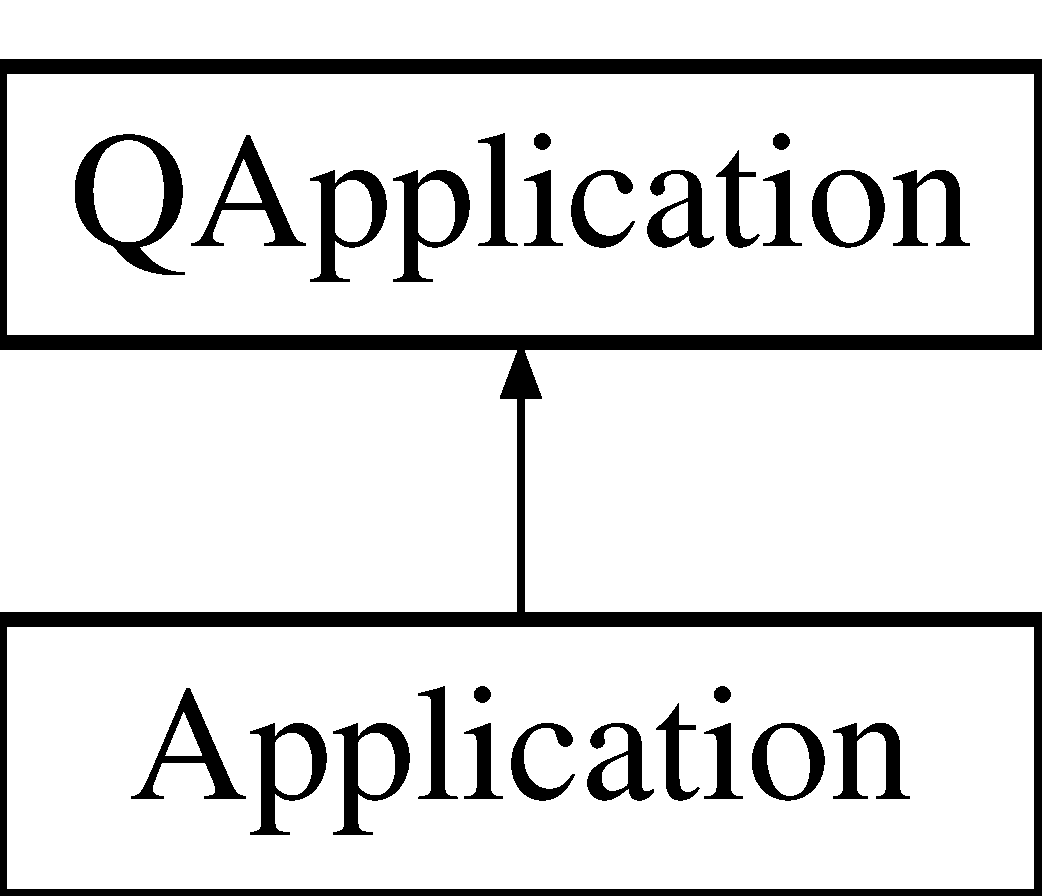
\includegraphics[height=2.000000cm]{classApplication}
\end{center}
\end{figure}
\subsection*{Public Member Functions}
\begin{DoxyCompactItemize}
\item 
\hypertarget{classApplication_a6e443cbe3481a06d8effb4fa8878499c}{{\bfseries Application} (int \&argc, char $\ast$$\ast$argv)}\label{classApplication_a6e443cbe3481a06d8effb4fa8878499c}

\item 
\hypertarget{classApplication_a566d9d9262f143093ce79c6e528fb584}{virtual bool {\bfseries notify} (Q\-Object $\ast$receiver, Q\-Event $\ast$event)}\label{classApplication_a566d9d9262f143093ce79c6e528fb584}

\end{DoxyCompactItemize}


The documentation for this class was generated from the following files\-:\begin{DoxyCompactItemize}
\item 
/home/jose/\-Documents/\-Seeded\-Image\-Segmentation\-Project/src/gui/application.\-h\item 
/home/jose/\-Documents/\-Seeded\-Image\-Segmentation\-Project/src/gui/application.\-cpp\end{DoxyCompactItemize}

\hypertarget{classDisplayWindow}{\section{Display\-Window Class Reference}
\label{classDisplayWindow}\index{Display\-Window@{Display\-Window}}
}


{\ttfamily \#include $<$displaywindow.\-h$>$}

Inheritance diagram for Display\-Window\-:\begin{figure}[H]
\begin{center}
\leavevmode
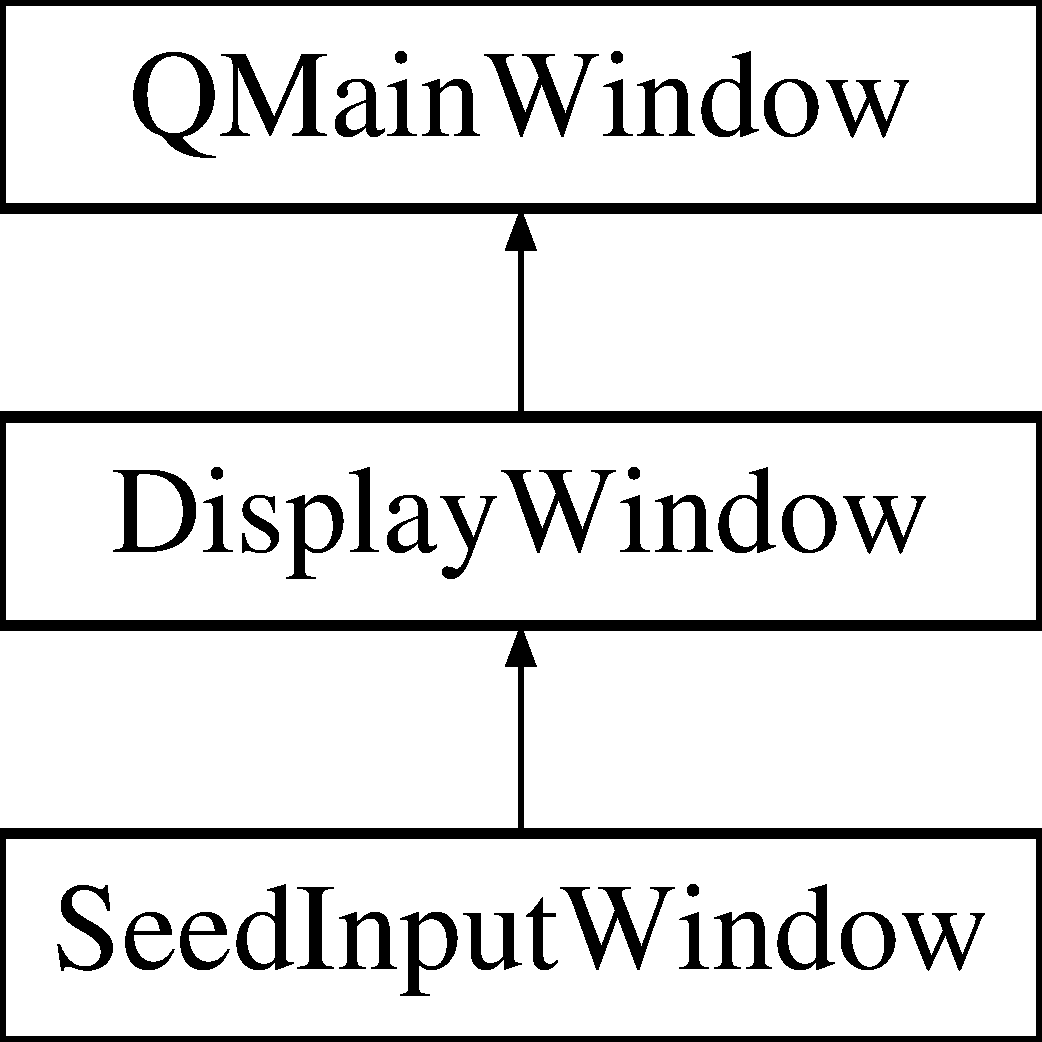
\includegraphics[height=3.000000cm]{classDisplayWindow}
\end{center}
\end{figure}
\subsection*{Public Member Functions}
\begin{DoxyCompactItemize}
\item 
\hyperlink{classDisplayWindow_abdc9ed2ae00b02f263498ad531e42bfa}{Display\-Window} ()
\item 
\hyperlink{classDisplayWindow_ae44d40aa2b4adb94332da5808fb5332c}{$\sim$\-Display\-Window} ()
\item 
void \hyperlink{classDisplayWindow_a8d29e0e63579cc008baf229b198ca144}{display\-Image} (const Q\-Image \&\hyperlink{classDisplayWindow_a312f36e9747e7f82d7b17be01429f69f}{image})
\item 
void \hyperlink{classDisplayWindow_aa01dee8e55e43adbab359d6de0ee9d4b}{paint\-Event} (Q\-Paint\-Event $\ast$event)
\end{DoxyCompactItemize}
\subsection*{Protected Attributes}
\begin{DoxyCompactItemize}
\item 
Q\-Image \hyperlink{classDisplayWindow_a312f36e9747e7f82d7b17be01429f69f}{image}
\end{DoxyCompactItemize}


\subsection{Detailed Description}
Class in charge of displaying the images on a window.

\begin{DoxySeeAlso}{See Also}
Karl Phillip, \href{https://github.com/karlphillip/GraphicsProgramming}{\tt https\-://github.\-com/karlphillip/\-Graphics\-Programming}
\end{DoxySeeAlso}
\begin{DoxyAuthor}{Author}
Rodrigo Daudt 
\end{DoxyAuthor}


\subsection{Constructor \& Destructor Documentation}
\hypertarget{classDisplayWindow_abdc9ed2ae00b02f263498ad531e42bfa}{\index{Display\-Window@{Display\-Window}!Display\-Window@{Display\-Window}}
\index{Display\-Window@{Display\-Window}!DisplayWindow@{Display\-Window}}
\subsubsection[{Display\-Window}]{\setlength{\rightskip}{0pt plus 5cm}Display\-Window\-::\-Display\-Window (
\begin{DoxyParamCaption}
{}
\end{DoxyParamCaption}
)}}\label{classDisplayWindow_abdc9ed2ae00b02f263498ad531e42bfa}
Default constructor. \hypertarget{classDisplayWindow_ae44d40aa2b4adb94332da5808fb5332c}{\index{Display\-Window@{Display\-Window}!$\sim$\-Display\-Window@{$\sim$\-Display\-Window}}
\index{$\sim$\-Display\-Window@{$\sim$\-Display\-Window}!DisplayWindow@{Display\-Window}}
\subsubsection[{$\sim$\-Display\-Window}]{\setlength{\rightskip}{0pt plus 5cm}Display\-Window\-::$\sim$\-Display\-Window (
\begin{DoxyParamCaption}
{}
\end{DoxyParamCaption}
)}}\label{classDisplayWindow_ae44d40aa2b4adb94332da5808fb5332c}
Class destructor. 

\subsection{Member Function Documentation}
\hypertarget{classDisplayWindow_a8d29e0e63579cc008baf229b198ca144}{\index{Display\-Window@{Display\-Window}!display\-Image@{display\-Image}}
\index{display\-Image@{display\-Image}!DisplayWindow@{Display\-Window}}
\subsubsection[{display\-Image}]{\setlength{\rightskip}{0pt plus 5cm}void Display\-Window\-::display\-Image (
\begin{DoxyParamCaption}
\item[{const Q\-Image \&}]{image}
\end{DoxyParamCaption}
)}}\label{classDisplayWindow_a8d29e0e63579cc008baf229b198ca144}
Displays the given Q\-Image.


\begin{DoxyParams}{Parameters}
{\em image} & image to be displayed. \\
\hline
\end{DoxyParams}
\hypertarget{classDisplayWindow_aa01dee8e55e43adbab359d6de0ee9d4b}{\index{Display\-Window@{Display\-Window}!paint\-Event@{paint\-Event}}
\index{paint\-Event@{paint\-Event}!DisplayWindow@{Display\-Window}}
\subsubsection[{paint\-Event}]{\setlength{\rightskip}{0pt plus 5cm}void Display\-Window\-::paint\-Event (
\begin{DoxyParamCaption}
\item[{Q\-Paint\-Event $\ast$}]{event}
\end{DoxyParamCaption}
)}}\label{classDisplayWindow_aa01dee8e55e43adbab359d6de0ee9d4b}
Handles the paint events


\begin{DoxyParams}{Parameters}
{\em event} & event triggered \\
\hline
\end{DoxyParams}


\subsection{Member Data Documentation}
\hypertarget{classDisplayWindow_a312f36e9747e7f82d7b17be01429f69f}{\index{Display\-Window@{Display\-Window}!image@{image}}
\index{image@{image}!DisplayWindow@{Display\-Window}}
\subsubsection[{image}]{\setlength{\rightskip}{0pt plus 5cm}Q\-Image Display\-Window\-::image\hspace{0.3cm}{\ttfamily [protected]}}}\label{classDisplayWindow_a312f36e9747e7f82d7b17be01429f69f}
Displayed image 

The documentation for this class was generated from the following files\-:\begin{DoxyCompactItemize}
\item 
/home/jose/\-Documents/\-Seeded\-Image\-Segmentation\-Project/src/gui/displaywindow.\-h\item 
/home/jose/\-Documents/\-Seeded\-Image\-Segmentation\-Project/src/gui/displaywindow.\-cpp\end{DoxyCompactItemize}

\hypertarget{classException}{\section{Exception Class Reference}
\label{classException}\index{Exception@{Exception}}
}


{\ttfamily \#include $<$exception.\-h$>$}

Inheritance diagram for Exception\-:\begin{figure}[H]
\begin{center}
\leavevmode
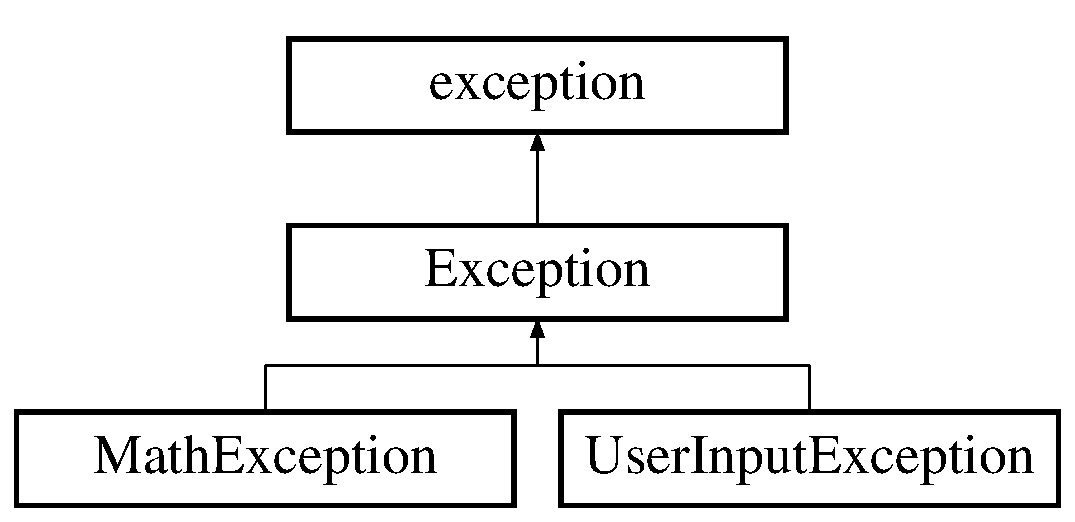
\includegraphics[height=3.000000cm]{classException}
\end{center}
\end{figure}
\subsection*{Public Member Functions}
\begin{DoxyCompactItemize}
\item 
\hyperlink{classException_a9509cd7ac8060afe83e6a483a5037305}{Exception} (const string \hyperlink{classException_adcb29a6ce336e7223a521e19cbd286a7}{name}, const string \hyperlink{classException_a3d5051a55e7133196d3097a5cd2d58a7}{message})
\item 
virtual \hyperlink{classException_ad1ba411de295ef2eeb02ba26284a829a}{$\sim$\-Exception} ()  throw ()
\item 
virtual const char $\ast$ \hyperlink{classException_a78154a31544a609cbd226d32574f52cd}{what} () const   throw ()
\end{DoxyCompactItemize}
\subsection*{Protected Attributes}
\begin{DoxyCompactItemize}
\item 
const string \hyperlink{classException_adcb29a6ce336e7223a521e19cbd286a7}{name}
\item 
const string \hyperlink{classException_a3d5051a55e7133196d3097a5cd2d58a7}{message}
\end{DoxyCompactItemize}


\subsection{Detailed Description}
This class represents the exceptions that can be in the app. Every exception class should inherit from this one.

\begin{DoxyAuthor}{Author}
Jose Bernal 
\end{DoxyAuthor}


\subsection{Constructor \& Destructor Documentation}
\hypertarget{classException_a9509cd7ac8060afe83e6a483a5037305}{\index{Exception@{Exception}!Exception@{Exception}}
\index{Exception@{Exception}!Exception@{Exception}}
\subsubsection[{Exception}]{\setlength{\rightskip}{0pt plus 5cm}Exception\-::\-Exception (
\begin{DoxyParamCaption}
\item[{const string}]{name, }
\item[{const string}]{message}
\end{DoxyParamCaption}
)}}\label{classException_a9509cd7ac8060afe83e6a483a5037305}
Default class constructor


\begin{DoxyParams}{Parameters}
{\em name} & Name of the exception \\
\hline
{\em message} & Message to display \\
\hline
\end{DoxyParams}
\hypertarget{classException_ad1ba411de295ef2eeb02ba26284a829a}{\index{Exception@{Exception}!$\sim$\-Exception@{$\sim$\-Exception}}
\index{$\sim$\-Exception@{$\sim$\-Exception}!Exception@{Exception}}
\subsubsection[{$\sim$\-Exception}]{\setlength{\rightskip}{0pt plus 5cm}virtual Exception\-::$\sim$\-Exception (
\begin{DoxyParamCaption}
{}
\end{DoxyParamCaption}
) throw  ) \hspace{0.3cm}{\ttfamily [inline]}, {\ttfamily [virtual]}}}\label{classException_ad1ba411de295ef2eeb02ba26284a829a}
Default destructor 

\subsection{Member Function Documentation}
\hypertarget{classException_a78154a31544a609cbd226d32574f52cd}{\index{Exception@{Exception}!what@{what}}
\index{what@{what}!Exception@{Exception}}
\subsubsection[{what}]{\setlength{\rightskip}{0pt plus 5cm}virtual const char$\ast$ Exception\-::what (
\begin{DoxyParamCaption}
{}
\end{DoxyParamCaption}
) const throw  ) \hspace{0.3cm}{\ttfamily [inline]}, {\ttfamily [virtual]}}}\label{classException_a78154a31544a609cbd226d32574f52cd}
Inherited 

\subsection{Member Data Documentation}
\hypertarget{classException_a3d5051a55e7133196d3097a5cd2d58a7}{\index{Exception@{Exception}!message@{message}}
\index{message@{message}!Exception@{Exception}}
\subsubsection[{message}]{\setlength{\rightskip}{0pt plus 5cm}const string Exception\-::message\hspace{0.3cm}{\ttfamily [protected]}}}\label{classException_a3d5051a55e7133196d3097a5cd2d58a7}
Message to display \hypertarget{classException_adcb29a6ce336e7223a521e19cbd286a7}{\index{Exception@{Exception}!name@{name}}
\index{name@{name}!Exception@{Exception}}
\subsubsection[{name}]{\setlength{\rightskip}{0pt plus 5cm}const string Exception\-::name\hspace{0.3cm}{\ttfamily [protected]}}}\label{classException_adcb29a6ce336e7223a521e19cbd286a7}
Name of the exception to display 

The documentation for this class was generated from the following files\-:\begin{DoxyCompactItemize}
\item 
/home/jose/\-Documents/\-Seeded\-Image\-Segmentation\-Project/src/exceptions/exception.\-h\item 
/home/jose/\-Documents/\-Seeded\-Image\-Segmentation\-Project/src/exceptions/exception.\-cpp\end{DoxyCompactItemize}

\hypertarget{classImageTypeConverter}{\section{Image\-Type\-Converter Class Reference}
\label{classImageTypeConverter}\index{Image\-Type\-Converter@{Image\-Type\-Converter}}
}


{\ttfamily \#include $<$imagetypeconverter.\-h$>$}

\subsection*{Static Public Member Functions}
\begin{DoxyCompactItemize}
\item 
static Mat \hyperlink{classImageTypeConverter_aa718633cbb8411411767128ced0c0442}{convert\-Q\-Image2\-Mat} (const Q\-Image \&image)
\item 
static Q\-Image \hyperlink{classImageTypeConverter_aaadc734d91c55e154619fa85a5a426ae}{convert\-Mat2\-Q\-Image} (const Mat \&image)
\end{DoxyCompactItemize}


\subsection{Detailed Description}
This class present a set of funtionalities for converting images from one variable type to another. Ej\-: Q\-Image -\/$>$ Mat

\begin{DoxyAuthor}{Author}
Jose Bernal 
\end{DoxyAuthor}


\subsection{Member Function Documentation}
\hypertarget{classImageTypeConverter_aaadc734d91c55e154619fa85a5a426ae}{\index{Image\-Type\-Converter@{Image\-Type\-Converter}!convert\-Mat2\-Q\-Image@{convert\-Mat2\-Q\-Image}}
\index{convert\-Mat2\-Q\-Image@{convert\-Mat2\-Q\-Image}!ImageTypeConverter@{Image\-Type\-Converter}}
\subsubsection[{convert\-Mat2\-Q\-Image}]{\setlength{\rightskip}{0pt plus 5cm}Q\-Image Image\-Type\-Converter\-::convert\-Mat2\-Q\-Image (
\begin{DoxyParamCaption}
\item[{const Mat \&}]{image}
\end{DoxyParamCaption}
)\hspace{0.3cm}{\ttfamily [static]}}}\label{classImageTypeConverter_aaadc734d91c55e154619fa85a5a426ae}
Converts a cv\-::\-Mat object to Q\-Image


\begin{DoxyParams}{Parameters}
{\em image} & cv\-::\-Mat object to convert\\
\hline
\end{DoxyParams}
\begin{DoxyReturn}{Returns}
the converted Q\-Image object
\end{DoxyReturn}
\begin{DoxySeeAlso}{See Also}
\href{http://answers.opencv.org/question/9075/how-do-i-save-qimage-in-cvmat/}{\tt http\-://answers.\-opencv.\-org/question/9075/how-\/do-\/i-\/save-\/qimage-\/in-\/cvmat/} 
\end{DoxySeeAlso}
\hypertarget{classImageTypeConverter_aa718633cbb8411411767128ced0c0442}{\index{Image\-Type\-Converter@{Image\-Type\-Converter}!convert\-Q\-Image2\-Mat@{convert\-Q\-Image2\-Mat}}
\index{convert\-Q\-Image2\-Mat@{convert\-Q\-Image2\-Mat}!ImageTypeConverter@{Image\-Type\-Converter}}
\subsubsection[{convert\-Q\-Image2\-Mat}]{\setlength{\rightskip}{0pt plus 5cm}Mat Image\-Type\-Converter\-::convert\-Q\-Image2\-Mat (
\begin{DoxyParamCaption}
\item[{const Q\-Image \&}]{image}
\end{DoxyParamCaption}
)\hspace{0.3cm}{\ttfamily [static]}}}\label{classImageTypeConverter_aa718633cbb8411411767128ced0c0442}
Converts a Q\-Image object to cv\-::\-Mat


\begin{DoxyParams}{Parameters}
{\em image} & Q\-Image object to convert\\
\hline
\end{DoxyParams}
\begin{DoxyReturn}{Returns}
the converted cv\-::\-Mat object
\end{DoxyReturn}
\begin{DoxySeeAlso}{See Also}
\href{http://answers.opencv.org/question/9075/how-do-i-save-qimage-in-cvmat/}{\tt http\-://answers.\-opencv.\-org/question/9075/how-\/do-\/i-\/save-\/qimage-\/in-\/cvmat/} 
\end{DoxySeeAlso}


The documentation for this class was generated from the following files\-:\begin{DoxyCompactItemize}
\item 
/home/jose/\-Documents/\-Seeded\-Image\-Segmentation\-Project/src/common/imagetypeconverter.\-h\item 
/home/jose/\-Documents/\-Seeded\-Image\-Segmentation\-Project/src/common/imagetypeconverter.\-cpp\end{DoxyCompactItemize}

\hypertarget{classMainWindow}{\section{Main\-Window Class Reference}
\label{classMainWindow}\index{Main\-Window@{Main\-Window}}
}


{\ttfamily \#include $<$mainwindow.\-h$>$}

Inheritance diagram for Main\-Window\-:\begin{figure}[H]
\begin{center}
\leavevmode
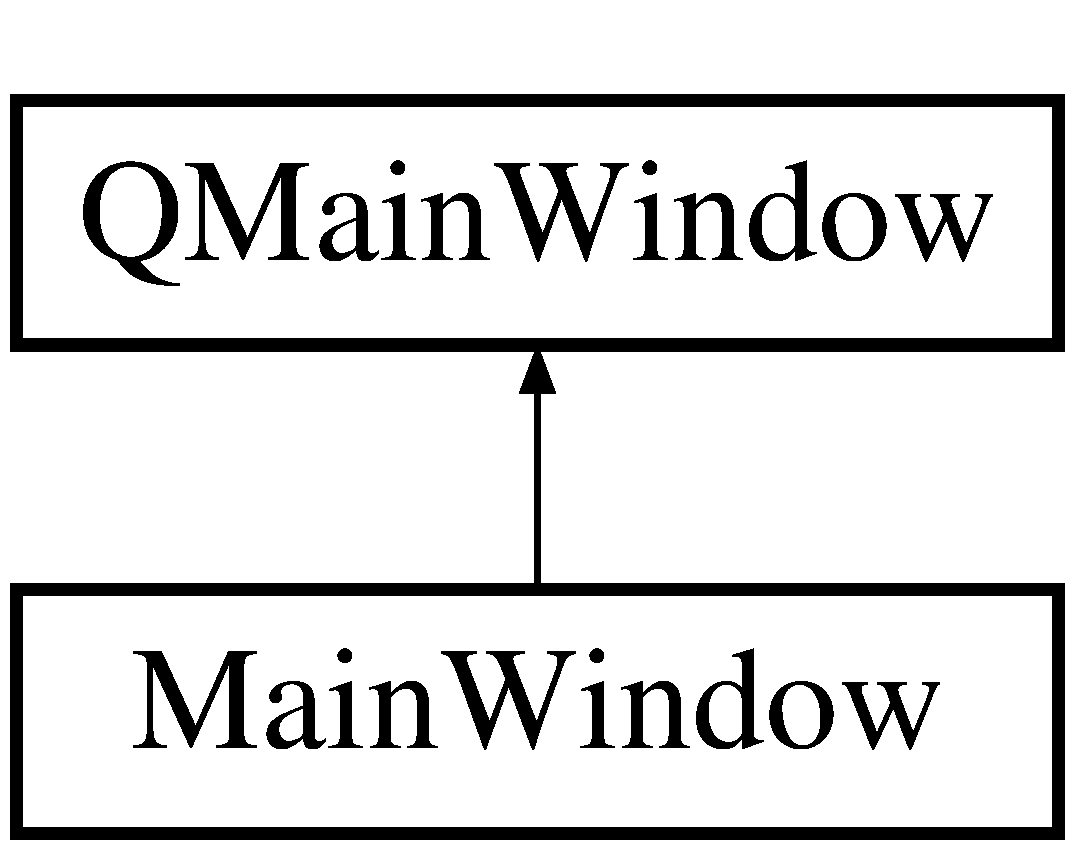
\includegraphics[height=2.000000cm]{classMainWindow}
\end{center}
\end{figure}
\subsection*{Public Member Functions}
\begin{DoxyCompactItemize}
\item 
\hyperlink{classMainWindow_a8b244be8b7b7db1b08de2a2acb9409db}{Main\-Window} (Q\-Widget $\ast$parent=0)
\item 
\hyperlink{classMainWindow_ae98d00a93bc118200eeef9f9bba1dba7}{$\sim$\-Main\-Window} ()
\end{DoxyCompactItemize}


\subsection{Detailed Description}
Main window of the application.

\begin{DoxyAuthor}{Author}
Rodrigo Daudt 
\end{DoxyAuthor}


\subsection{Constructor \& Destructor Documentation}
\hypertarget{classMainWindow_a8b244be8b7b7db1b08de2a2acb9409db}{\index{Main\-Window@{Main\-Window}!Main\-Window@{Main\-Window}}
\index{Main\-Window@{Main\-Window}!MainWindow@{Main\-Window}}
\subsubsection[{Main\-Window}]{\setlength{\rightskip}{0pt plus 5cm}Main\-Window\-::\-Main\-Window (
\begin{DoxyParamCaption}
\item[{Q\-Widget $\ast$}]{parent = {\ttfamily 0}}
\end{DoxyParamCaption}
)\hspace{0.3cm}{\ttfamily [explicit]}}}\label{classMainWindow_a8b244be8b7b7db1b08de2a2acb9409db}
Default constructor


\begin{DoxyParams}{Parameters}
{\em parent} & parent component \\
\hline
\end{DoxyParams}
\hypertarget{classMainWindow_ae98d00a93bc118200eeef9f9bba1dba7}{\index{Main\-Window@{Main\-Window}!$\sim$\-Main\-Window@{$\sim$\-Main\-Window}}
\index{$\sim$\-Main\-Window@{$\sim$\-Main\-Window}!MainWindow@{Main\-Window}}
\subsubsection[{$\sim$\-Main\-Window}]{\setlength{\rightskip}{0pt plus 5cm}Main\-Window\-::$\sim$\-Main\-Window (
\begin{DoxyParamCaption}
{}
\end{DoxyParamCaption}
)}}\label{classMainWindow_ae98d00a93bc118200eeef9f9bba1dba7}
Class destructor. 

The documentation for this class was generated from the following files\-:\begin{DoxyCompactItemize}
\item 
/home/jose/\-Documents/\-Seeded\-Image\-Segmentation\-Project/src/gui/mainwindow.\-h\item 
/home/jose/\-Documents/\-Seeded\-Image\-Segmentation\-Project/src/gui/mainwindow.\-cpp\end{DoxyCompactItemize}

\hypertarget{classUi_1_1MainWindow}{\section{Ui\-:\-:Main\-Window Class Reference}
\label{classUi_1_1MainWindow}\index{Ui\-::\-Main\-Window@{Ui\-::\-Main\-Window}}
}
Inheritance diagram for Ui\-:\-:Main\-Window\-:\begin{figure}[H]
\begin{center}
\leavevmode
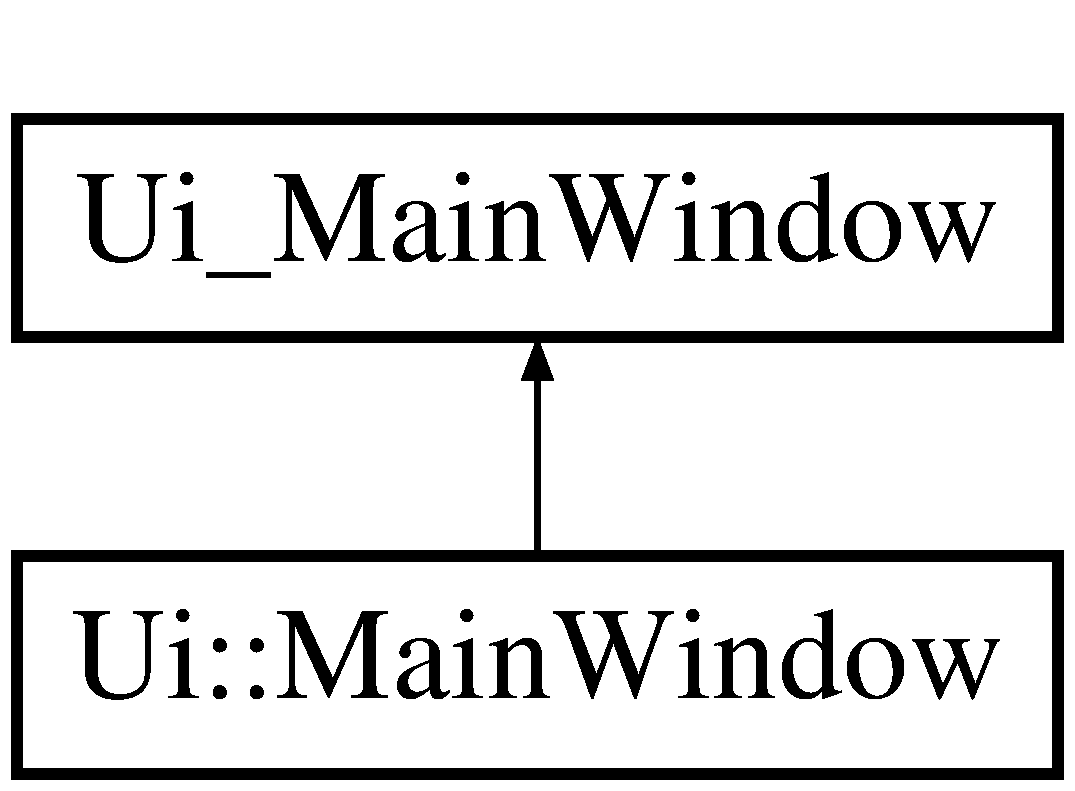
\includegraphics[height=2.000000cm]{classUi_1_1MainWindow}
\end{center}
\end{figure}
\subsection*{Additional Inherited Members}


The documentation for this class was generated from the following file\-:\begin{DoxyCompactItemize}
\item 
/home/jose/\-Documents/\-Seeded\-Image\-Segmentation\-Project/src/gui/ui\-\_\-mainwindow.\-h\end{DoxyCompactItemize}

\hypertarget{classMathException}{\section{Math\-Exception Class Reference}
\label{classMathException}\index{Math\-Exception@{Math\-Exception}}
}


{\ttfamily \#include $<$mathexception.\-h$>$}

Inheritance diagram for Math\-Exception\-:\begin{figure}[H]
\begin{center}
\leavevmode
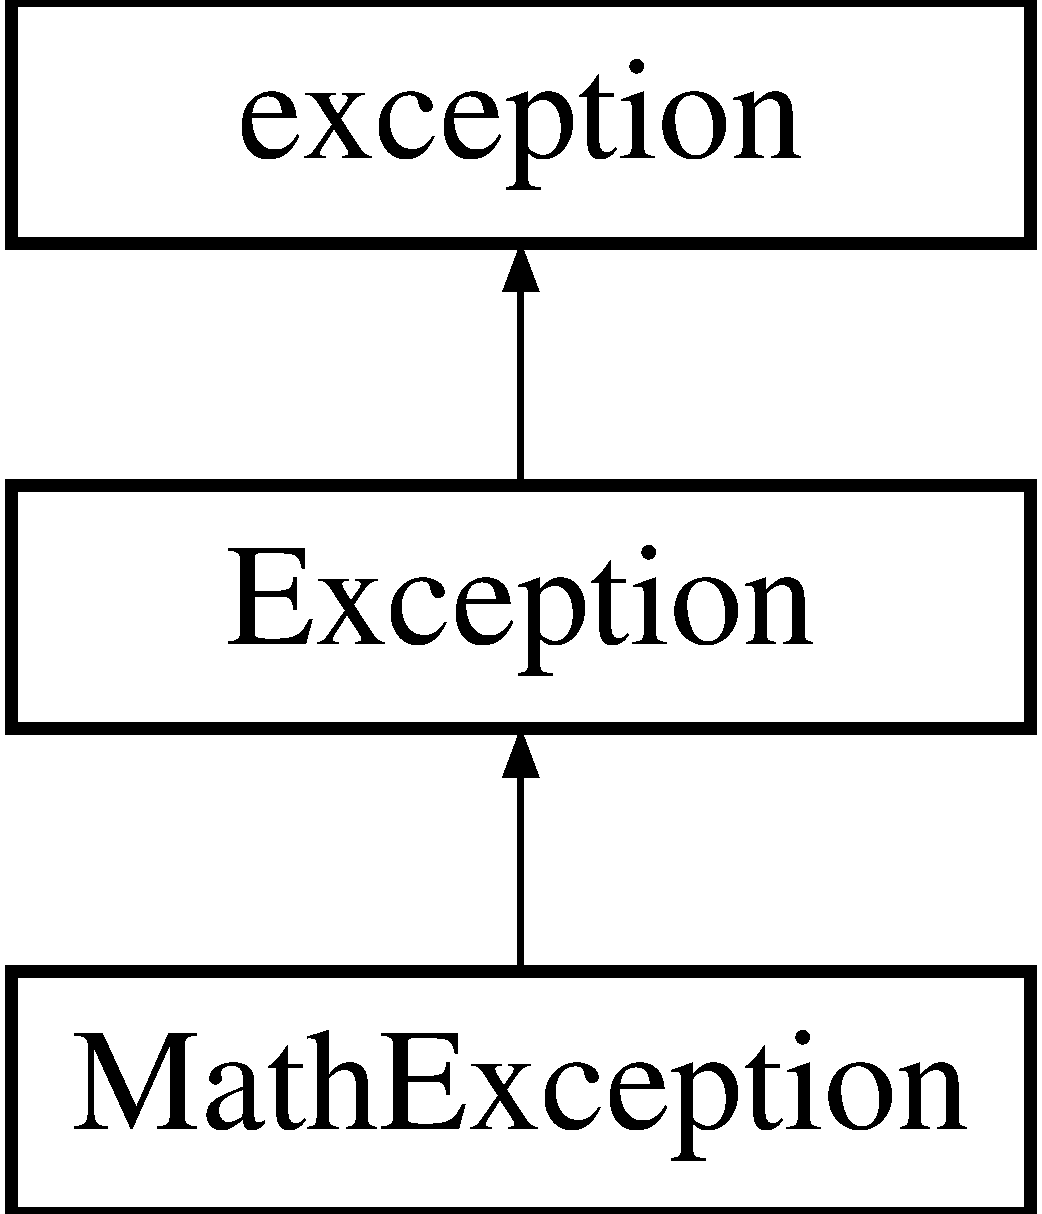
\includegraphics[height=3.000000cm]{classMathException}
\end{center}
\end{figure}
\subsection*{Public Member Functions}
\begin{DoxyCompactItemize}
\item 
\hyperlink{classMathException_aa4254eabcd2e2f9b2bfd90f9fb6280c2}{Math\-Exception} (const string \hyperlink{classException_a3d5051a55e7133196d3097a5cd2d58a7}{message})
\end{DoxyCompactItemize}
\subsection*{Additional Inherited Members}


\subsection{Detailed Description}
This class represents the mathematical exceptions that have place in the app.

\begin{DoxyAuthor}{Author}
Jose Bernal 
\end{DoxyAuthor}


\subsection{Constructor \& Destructor Documentation}
\hypertarget{classMathException_aa4254eabcd2e2f9b2bfd90f9fb6280c2}{\index{Math\-Exception@{Math\-Exception}!Math\-Exception@{Math\-Exception}}
\index{Math\-Exception@{Math\-Exception}!MathException@{Math\-Exception}}
\subsubsection[{Math\-Exception}]{\setlength{\rightskip}{0pt plus 5cm}Math\-Exception\-::\-Math\-Exception (
\begin{DoxyParamCaption}
\item[{const string}]{message}
\end{DoxyParamCaption}
)}}\label{classMathException_aa4254eabcd2e2f9b2bfd90f9fb6280c2}
Default constructor of the class


\begin{DoxyParams}{Parameters}
{\em message} & Message to display \\
\hline
\end{DoxyParams}


The documentation for this class was generated from the following files\-:\begin{DoxyCompactItemize}
\item 
/home/jose/\-Documents/\-Seeded\-Image\-Segmentation\-Project/src/exceptions/mathexception.\-h\item 
/home/jose/\-Documents/\-Seeded\-Image\-Segmentation\-Project/src/exceptions/mathexception.\-cpp\end{DoxyCompactItemize}

\hypertarget{classNeighbourhood}{\section{Neighbourhood Class Reference}
\label{classNeighbourhood}\index{Neighbourhood@{Neighbourhood}}
}


{\ttfamily \#include $<$neighbourhood.\-h$>$}

\subsection*{Public Member Functions}
\begin{DoxyCompactItemize}
\item 
\hyperlink{classNeighbourhood_a1fafe62e922347ad822d30f9d861781f}{Neighbourhood} ()
\item 
\hyperlink{classNeighbourhood_af236d52391c0628820fb3cc3fa9eaeaf}{Neighbourhood} (const vector$<$ Point2i $>$ \&neighbour\-Positions)
\item 
\hyperlink{classNeighbourhood_a4df78b0d75b48ed2ed880eb7d68f7a61}{$\sim$\-Neighbourhood} ()
\item 
Point2i \hyperlink{classNeighbourhood_aaa685395d5e4a0783cd7a1a4e8759a60}{operator()} (const unsigned int idx) const 
\item 
unsigned int \hyperlink{classNeighbourhood_a5cdb16c3679f68d4e8de510276be1051}{size} () const 
\end{DoxyCompactItemize}


\subsection{Detailed Description}
This class represents a neighbourhood of size rows x cols. The pixels in the neighbourhood are by default inactive. Thus, the pixels to consider in the neighbourhood should be set to active.

\begin{DoxyAuthor}{Author}
Jose Bernal 
\end{DoxyAuthor}


\subsection{Constructor \& Destructor Documentation}
\hypertarget{classNeighbourhood_a1fafe62e922347ad822d30f9d861781f}{\index{Neighbourhood@{Neighbourhood}!Neighbourhood@{Neighbourhood}}
\index{Neighbourhood@{Neighbourhood}!Neighbourhood@{Neighbourhood}}
\subsubsection[{Neighbourhood}]{\setlength{\rightskip}{0pt plus 5cm}Neighbourhood\-::\-Neighbourhood (
\begin{DoxyParamCaption}
{}
\end{DoxyParamCaption}
)}}\label{classNeighbourhood_a1fafe62e922347ad822d30f9d861781f}
Default constructor \hypertarget{classNeighbourhood_af236d52391c0628820fb3cc3fa9eaeaf}{\index{Neighbourhood@{Neighbourhood}!Neighbourhood@{Neighbourhood}}
\index{Neighbourhood@{Neighbourhood}!Neighbourhood@{Neighbourhood}}
\subsubsection[{Neighbourhood}]{\setlength{\rightskip}{0pt plus 5cm}Neighbourhood\-::\-Neighbourhood (
\begin{DoxyParamCaption}
\item[{const vector$<$ Point2i $>$ \&}]{neighbour\-Positions}
\end{DoxyParamCaption}
)}}\label{classNeighbourhood_af236d52391c0628820fb3cc3fa9eaeaf}
Parametrized constructor


\begin{DoxyParams}{Parameters}
{\em neighbour\-Positions} & neighbour positions to take into account. \\
\hline
\end{DoxyParams}
\hypertarget{classNeighbourhood_a4df78b0d75b48ed2ed880eb7d68f7a61}{\index{Neighbourhood@{Neighbourhood}!$\sim$\-Neighbourhood@{$\sim$\-Neighbourhood}}
\index{$\sim$\-Neighbourhood@{$\sim$\-Neighbourhood}!Neighbourhood@{Neighbourhood}}
\subsubsection[{$\sim$\-Neighbourhood}]{\setlength{\rightskip}{0pt plus 5cm}Neighbourhood\-::$\sim$\-Neighbourhood (
\begin{DoxyParamCaption}
{}
\end{DoxyParamCaption}
)}}\label{classNeighbourhood_a4df78b0d75b48ed2ed880eb7d68f7a61}
Class destructor 

\subsection{Member Function Documentation}
\hypertarget{classNeighbourhood_aaa685395d5e4a0783cd7a1a4e8759a60}{\index{Neighbourhood@{Neighbourhood}!operator()@{operator()}}
\index{operator()@{operator()}!Neighbourhood@{Neighbourhood}}
\subsubsection[{operator()}]{\setlength{\rightskip}{0pt plus 5cm}Point2i Neighbourhood\-::operator() (
\begin{DoxyParamCaption}
\item[{const unsigned int}]{idx}
\end{DoxyParamCaption}
) const}}\label{classNeighbourhood_aaa685395d5e4a0783cd7a1a4e8759a60}
Returns the neighbour position at the index idx. If the idx is out of bounds, an \hyperlink{classUserInputException}{User\-Input\-Exception} is thrown.


\begin{DoxyParams}{Parameters}
{\em idx} & index of the neighbour position to get\\
\hline
\end{DoxyParams}
\begin{DoxyReturn}{Returns}
the position of the idx-\/th neighbour 
\end{DoxyReturn}
\hypertarget{classNeighbourhood_a5cdb16c3679f68d4e8de510276be1051}{\index{Neighbourhood@{Neighbourhood}!size@{size}}
\index{size@{size}!Neighbourhood@{Neighbourhood}}
\subsubsection[{size}]{\setlength{\rightskip}{0pt plus 5cm}unsigned int Neighbourhood\-::size (
\begin{DoxyParamCaption}
{}
\end{DoxyParamCaption}
) const}}\label{classNeighbourhood_a5cdb16c3679f68d4e8de510276be1051}
Returns the size of the neighbourhood. If the neighbourhood is 3x3, the expected size is 8.

\begin{DoxyReturn}{Returns}
the size of the neightbourhood 
\end{DoxyReturn}


The documentation for this class was generated from the following files\-:\begin{DoxyCompactItemize}
\item 
/home/jose/\-Documents/\-Seeded\-Image\-Segmentation\-Project/src/common/neighbourhood.\-h\item 
/home/jose/\-Documents/\-Seeded\-Image\-Segmentation\-Project/src/common/neighbourhood.\-cpp\end{DoxyCompactItemize}

\hypertarget{classNeighbourhoodFactory}{\section{Neighbourhood\-Factory Class Reference}
\label{classNeighbourhoodFactory}\index{Neighbourhood\-Factory@{Neighbourhood\-Factory}}
}


{\ttfamily \#include $<$neighbourhoodfactory.\-h$>$}

\subsection*{Public Types}
\begin{DoxyCompactItemize}
\item 
enum \hyperlink{classNeighbourhoodFactory_a299ccbd341de315b0e7bf5cf868bf72b}{Neighbourhood\-Type} \{ {\bfseries N8}, 
{\bfseries N4}
 \}
\end{DoxyCompactItemize}
\subsection*{Static Public Member Functions}
\begin{DoxyCompactItemize}
\item 
static \hyperlink{classNeighbourhood}{Neighbourhood} \hyperlink{classNeighbourhoodFactory_a2d492970c0ba303bc2e9302ea03ee467}{create\-Neighbourhood} (const \hyperlink{classNeighbourhoodFactory_a299ccbd341de315b0e7bf5cf868bf72b}{Neighbourhood\-Type} type)
\end{DoxyCompactItemize}


\subsection{Detailed Description}
This factory class is in charge of generating instances of the Neighbourhoods. There are basically two types of neighbourhoods N8 (8 neighbours) and N4 (4 neighbours).

\begin{DoxyAuthor}{Author}
Jose Bernal 
\end{DoxyAuthor}


\subsection{Member Enumeration Documentation}
\hypertarget{classNeighbourhoodFactory_a299ccbd341de315b0e7bf5cf868bf72b}{\index{Neighbourhood\-Factory@{Neighbourhood\-Factory}!Neighbourhood\-Type@{Neighbourhood\-Type}}
\index{Neighbourhood\-Type@{Neighbourhood\-Type}!NeighbourhoodFactory@{Neighbourhood\-Factory}}
\subsubsection[{Neighbourhood\-Type}]{\setlength{\rightskip}{0pt plus 5cm}enum {\bf Neighbourhood\-Factory\-::\-Neighbourhood\-Type}}}\label{classNeighbourhoodFactory_a299ccbd341de315b0e7bf5cf868bf72b}
This enum represents the possible neighbourhood types that can be build using this factory class. Using N8 will create a 8-\/neighbours and N4 a 4-\/neighbours. 

\subsection{Member Function Documentation}
\hypertarget{classNeighbourhoodFactory_a2d492970c0ba303bc2e9302ea03ee467}{\index{Neighbourhood\-Factory@{Neighbourhood\-Factory}!create\-Neighbourhood@{create\-Neighbourhood}}
\index{create\-Neighbourhood@{create\-Neighbourhood}!NeighbourhoodFactory@{Neighbourhood\-Factory}}
\subsubsection[{create\-Neighbourhood}]{\setlength{\rightskip}{0pt plus 5cm}{\bf Neighbourhood} Neighbourhood\-Factory\-::create\-Neighbourhood (
\begin{DoxyParamCaption}
\item[{const {\bf Neighbourhood\-Type}}]{type}
\end{DoxyParamCaption}
)\hspace{0.3cm}{\ttfamily [static]}}}\label{classNeighbourhoodFactory_a2d492970c0ba303bc2e9302ea03ee467}
Creates the neighbourhood based on the given type.


\begin{DoxyParams}{Parameters}
{\em type} & the Neighbourhood\-Type to use\\
\hline
\end{DoxyParams}
\begin{DoxyReturn}{Returns}
a \hyperlink{classNeighbourhood}{Neighbourhood} instance of the given type 
\end{DoxyReturn}


The documentation for this class was generated from the following files\-:\begin{DoxyCompactItemize}
\item 
/home/jose/\-Documents/\-Seeded\-Image\-Segmentation\-Project/src/common/neighbourhoodfactory.\-h\item 
/home/jose/\-Documents/\-Seeded\-Image\-Segmentation\-Project/src/common/neighbourhoodfactory.\-cpp\end{DoxyCompactItemize}

\hypertarget{classSeededSegmentation}{\section{Seeded\-Segmentation Class Reference}
\label{classSeededSegmentation}\index{Seeded\-Segmentation@{Seeded\-Segmentation}}
}


{\ttfamily \#include $<$seededsegmentation.\-h$>$}

\subsection*{Public Member Functions}
\begin{DoxyCompactItemize}
\item 
\hyperlink{classSeededSegmentation_ae9b10d44de68a3975d392b7fb23ff741}{Seeded\-Segmentation} ()
\item 
\hyperlink{classSeededSegmentation_ad68f11e2aa003293fd279b5f75d57c08}{$\sim$\-Seeded\-Segmentation} ()
\item 
Mat \hyperlink{classSeededSegmentation_af089f8aa4f5d28a4c2c1085486502b94}{segment} (const Mat \&input\-Image, const Mat \&background\-Image, const Mat \&foreground\-Image, const \hyperlink{classNeighbourhood}{Neighbourhood} \&neighbourhood, const double beta, const double sigma=0.\-1)
\end{DoxyCompactItemize}


\subsection{Detailed Description}
This class segment a given input image using the laplacian seeded segmentation proposed for Casaca et al.

\begin{DoxySeeAlso}{See Also}
Laplacian Coordinates for Seeded Image Segmentation in \href{https://sites.google.com/site/wallacecoc/publications}{\tt https\-://sites.\-google.\-com/site/wallacecoc/publications}
\end{DoxySeeAlso}
\begin{DoxyAuthor}{Author}
Jose Bernal 
\end{DoxyAuthor}


\subsection{Constructor \& Destructor Documentation}
\hypertarget{classSeededSegmentation_ae9b10d44de68a3975d392b7fb23ff741}{\index{Seeded\-Segmentation@{Seeded\-Segmentation}!Seeded\-Segmentation@{Seeded\-Segmentation}}
\index{Seeded\-Segmentation@{Seeded\-Segmentation}!SeededSegmentation@{Seeded\-Segmentation}}
\subsubsection[{Seeded\-Segmentation}]{\setlength{\rightskip}{0pt plus 5cm}Seeded\-Segmentation\-::\-Seeded\-Segmentation (
\begin{DoxyParamCaption}
{}
\end{DoxyParamCaption}
)}}\label{classSeededSegmentation_ae9b10d44de68a3975d392b7fb23ff741}
Default constructor. \hypertarget{classSeededSegmentation_ad68f11e2aa003293fd279b5f75d57c08}{\index{Seeded\-Segmentation@{Seeded\-Segmentation}!$\sim$\-Seeded\-Segmentation@{$\sim$\-Seeded\-Segmentation}}
\index{$\sim$\-Seeded\-Segmentation@{$\sim$\-Seeded\-Segmentation}!SeededSegmentation@{Seeded\-Segmentation}}
\subsubsection[{$\sim$\-Seeded\-Segmentation}]{\setlength{\rightskip}{0pt plus 5cm}Seeded\-Segmentation\-::$\sim$\-Seeded\-Segmentation (
\begin{DoxyParamCaption}
{}
\end{DoxyParamCaption}
)}}\label{classSeededSegmentation_ad68f11e2aa003293fd279b5f75d57c08}
Class destructor 

\subsection{Member Function Documentation}
\hypertarget{classSeededSegmentation_af089f8aa4f5d28a4c2c1085486502b94}{\index{Seeded\-Segmentation@{Seeded\-Segmentation}!segment@{segment}}
\index{segment@{segment}!SeededSegmentation@{Seeded\-Segmentation}}
\subsubsection[{segment}]{\setlength{\rightskip}{0pt plus 5cm}Mat Seeded\-Segmentation\-::segment (
\begin{DoxyParamCaption}
\item[{const Mat \&}]{input\-Image, }
\item[{const Mat \&}]{background\-Image, }
\item[{const Mat \&}]{foreground\-Image, }
\item[{const {\bf Neighbourhood} \&}]{neighbourhood, }
\item[{const double}]{beta, }
\item[{const double}]{sigma = {\ttfamily 0.1}}
\end{DoxyParamCaption}
)}}\label{classSeededSegmentation_af089f8aa4f5d28a4c2c1085486502b94}
Segment method receives 2 matrixes of type Mat and returns the corresponding segmentation given the input, background and foreground images.


\begin{DoxyParams}{Parameters}
{\em input\-Image} & Image to be segmented. \\
\hline
{\em background\-Image} & Matrix Mat containing the background image. This matrix should contain 0 if the pixel belongs to the background and 1 otherwise. \\
\hline
{\em foreground\-Image} & Matrix Mat containing the foreground image. This matrix should contain 0 if the pixel belongs to the foreground and 1 otherwise. \\
\hline
{\em neighbourhood} & neighbourhood to use to calculate the laplacian matrix. \\
\hline
{\em beta} & corresponds to a tuning constant weighting the neighborhood \\
\hline
{\em sigma} & corresponds to the maximum value among the all diferences. A different value can be received but it should be positive.\\
\hline
\end{DoxyParams}
\begin{DoxyReturn}{Returns}
A binary matrix Mat containing the segmented image. This matrix will contain 0 if the pixel belongs to the foreground and 1 otherwise. 
\end{DoxyReturn}


The documentation for this class was generated from the following files\-:\begin{DoxyCompactItemize}
\item 
/home/jose/\-Documents/\-Seeded\-Image\-Segmentation\-Project/src/mathtools/seededsegmentation.\-h\item 
/home/jose/\-Documents/\-Seeded\-Image\-Segmentation\-Project/src/mathtools/seededsegmentation.\-cpp\end{DoxyCompactItemize}

\hypertarget{classSeedInputWindow}{\section{Seed\-Input\-Window Class Reference}
\label{classSeedInputWindow}\index{Seed\-Input\-Window@{Seed\-Input\-Window}}
}


{\ttfamily \#include $<$seedinputwindow.\-h$>$}

Inheritance diagram for Seed\-Input\-Window\-:\begin{figure}[H]
\begin{center}
\leavevmode
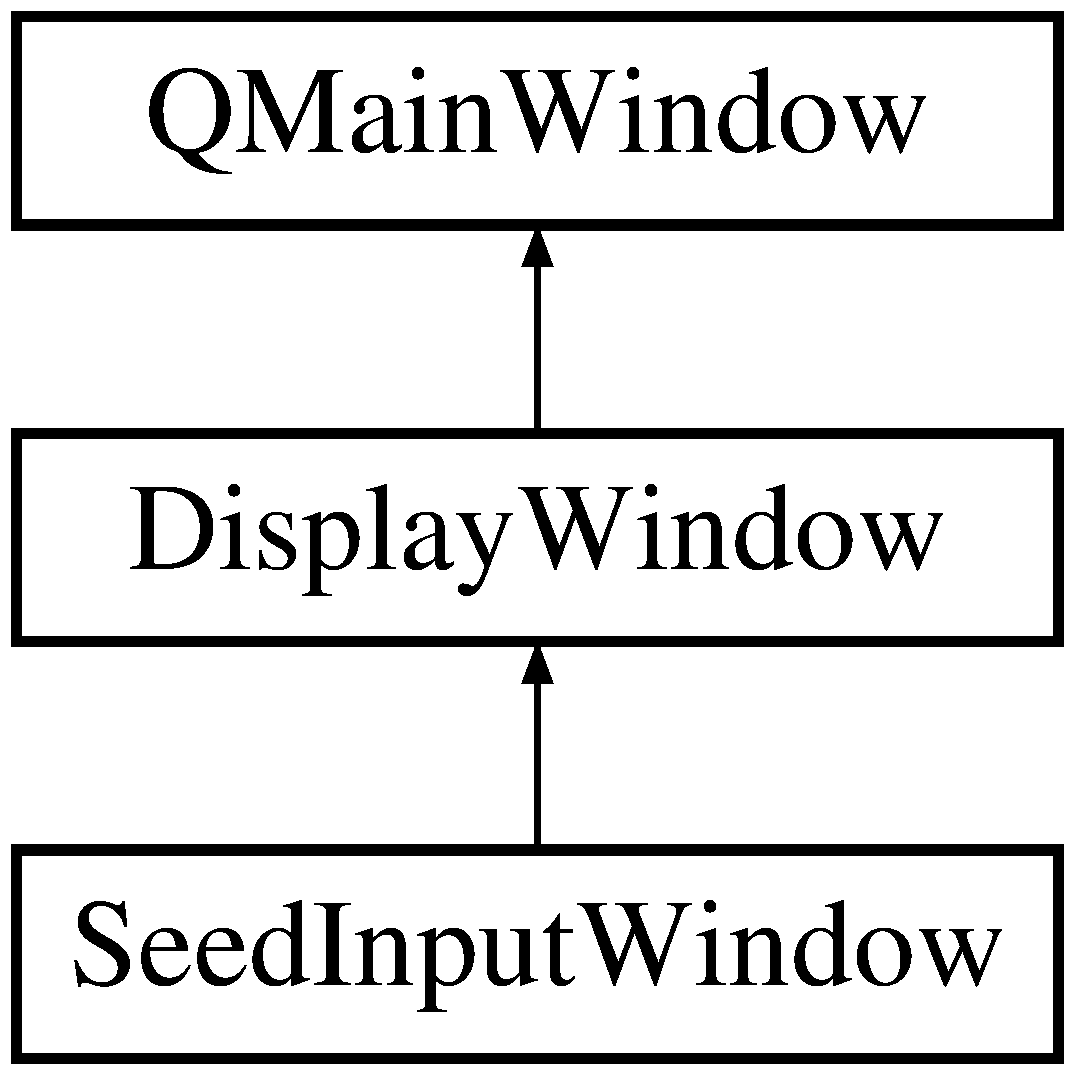
\includegraphics[height=3.000000cm]{classSeedInputWindow}
\end{center}
\end{figure}
\subsection*{Signals}
\begin{DoxyCompactItemize}
\item 
void \hyperlink{classSeedInputWindow_a71742a7b514dc88ef41db24e8c51043c}{update\-Pixel} (const unsigned int i, const unsigned int j)
\end{DoxyCompactItemize}
\subsection*{Public Member Functions}
\begin{DoxyCompactItemize}
\item 
\hyperlink{classSeedInputWindow_aa61c9965942eff3b348988c35e2375fe}{Seed\-Input\-Window} ()
\item 
\hyperlink{classSeedInputWindow_af6c2f37c19c6755afe654158a6e9baec}{$\sim$\-Seed\-Input\-Window} ()
\item 
void \hyperlink{classSeedInputWindow_a3c534db4845c26958f38651ec0560134}{set\-Seed\-Color} (const Q\-Rgb seed\-Color)
\item 
void \hyperlink{classSeedInputWindow_ac00157b8a7abc95014d1bba6191ae3c3}{mouse\-Move\-Event} (Q\-Mouse\-Event $\ast$event)
\end{DoxyCompactItemize}
\subsection*{Additional Inherited Members}


\subsection{Detailed Description}
Class in charge of input of segmentation seeds

\begin{DoxyAuthor}{Author}
Rodrigo Daudt 
\end{DoxyAuthor}


\subsection{Constructor \& Destructor Documentation}
\hypertarget{classSeedInputWindow_aa61c9965942eff3b348988c35e2375fe}{\index{Seed\-Input\-Window@{Seed\-Input\-Window}!Seed\-Input\-Window@{Seed\-Input\-Window}}
\index{Seed\-Input\-Window@{Seed\-Input\-Window}!SeedInputWindow@{Seed\-Input\-Window}}
\subsubsection[{Seed\-Input\-Window}]{\setlength{\rightskip}{0pt plus 5cm}Seed\-Input\-Window\-::\-Seed\-Input\-Window (
\begin{DoxyParamCaption}
{}
\end{DoxyParamCaption}
)}}\label{classSeedInputWindow_aa61c9965942eff3b348988c35e2375fe}
Default constructor. \hypertarget{classSeedInputWindow_af6c2f37c19c6755afe654158a6e9baec}{\index{Seed\-Input\-Window@{Seed\-Input\-Window}!$\sim$\-Seed\-Input\-Window@{$\sim$\-Seed\-Input\-Window}}
\index{$\sim$\-Seed\-Input\-Window@{$\sim$\-Seed\-Input\-Window}!SeedInputWindow@{Seed\-Input\-Window}}
\subsubsection[{$\sim$\-Seed\-Input\-Window}]{\setlength{\rightskip}{0pt plus 5cm}Seed\-Input\-Window\-::$\sim$\-Seed\-Input\-Window (
\begin{DoxyParamCaption}
{}
\end{DoxyParamCaption}
)}}\label{classSeedInputWindow_af6c2f37c19c6755afe654158a6e9baec}
Class destructor. 

\subsection{Member Function Documentation}
\hypertarget{classSeedInputWindow_ac00157b8a7abc95014d1bba6191ae3c3}{\index{Seed\-Input\-Window@{Seed\-Input\-Window}!mouse\-Move\-Event@{mouse\-Move\-Event}}
\index{mouse\-Move\-Event@{mouse\-Move\-Event}!SeedInputWindow@{Seed\-Input\-Window}}
\subsubsection[{mouse\-Move\-Event}]{\setlength{\rightskip}{0pt plus 5cm}void Seed\-Input\-Window\-::mouse\-Move\-Event (
\begin{DoxyParamCaption}
\item[{Q\-Mouse\-Event $\ast$}]{event}
\end{DoxyParamCaption}
)}}\label{classSeedInputWindow_ac00157b8a7abc95014d1bba6191ae3c3}
Handles the mouse move events


\begin{DoxyParams}{Parameters}
{\em event} & event triggered \\
\hline
\end{DoxyParams}
\hypertarget{classSeedInputWindow_a3c534db4845c26958f38651ec0560134}{\index{Seed\-Input\-Window@{Seed\-Input\-Window}!set\-Seed\-Color@{set\-Seed\-Color}}
\index{set\-Seed\-Color@{set\-Seed\-Color}!SeedInputWindow@{Seed\-Input\-Window}}
\subsubsection[{set\-Seed\-Color}]{\setlength{\rightskip}{0pt plus 5cm}void Seed\-Input\-Window\-::set\-Seed\-Color (
\begin{DoxyParamCaption}
\item[{const Q\-Rgb}]{seed\-Color}
\end{DoxyParamCaption}
)}}\label{classSeedInputWindow_a3c534db4845c26958f38651ec0560134}
Sets the color of the seed.


\begin{DoxyParams}{Parameters}
{\em seed\-Color} & seed color to use. \\
\hline
\end{DoxyParams}
\hypertarget{classSeedInputWindow_a71742a7b514dc88ef41db24e8c51043c}{\index{Seed\-Input\-Window@{Seed\-Input\-Window}!update\-Pixel@{update\-Pixel}}
\index{update\-Pixel@{update\-Pixel}!SeedInputWindow@{Seed\-Input\-Window}}
\subsubsection[{update\-Pixel}]{\setlength{\rightskip}{0pt plus 5cm}void Seed\-Input\-Window\-::update\-Pixel (
\begin{DoxyParamCaption}
\item[{const unsigned int}]{i, }
\item[{const unsigned int}]{j}
\end{DoxyParamCaption}
)\hspace{0.3cm}{\ttfamily [signal]}}}\label{classSeedInputWindow_a71742a7b514dc88ef41db24e8c51043c}
Signal emitted when a drawing the seeds. 

The documentation for this class was generated from the following files\-:\begin{DoxyCompactItemize}
\item 
/home/jose/\-Documents/\-Seeded\-Image\-Segmentation\-Project/src/gui/seedinputwindow.\-h\item 
/home/jose/\-Documents/\-Seeded\-Image\-Segmentation\-Project/src/gui/moc\-\_\-seedinputwindow.\-cpp\item 
/home/jose/\-Documents/\-Seeded\-Image\-Segmentation\-Project/src/gui/seedinputwindow.\-cpp\end{DoxyCompactItemize}

\hypertarget{classSegmentationEventHandler}{\section{Segmentation\-Event\-Handler Class Reference}
\label{classSegmentationEventHandler}\index{Segmentation\-Event\-Handler@{Segmentation\-Event\-Handler}}
}


{\ttfamily \#include $<$segmentationeventhandler.\-h$>$}

Inheritance diagram for Segmentation\-Event\-Handler\-:\begin{figure}[H]
\begin{center}
\leavevmode
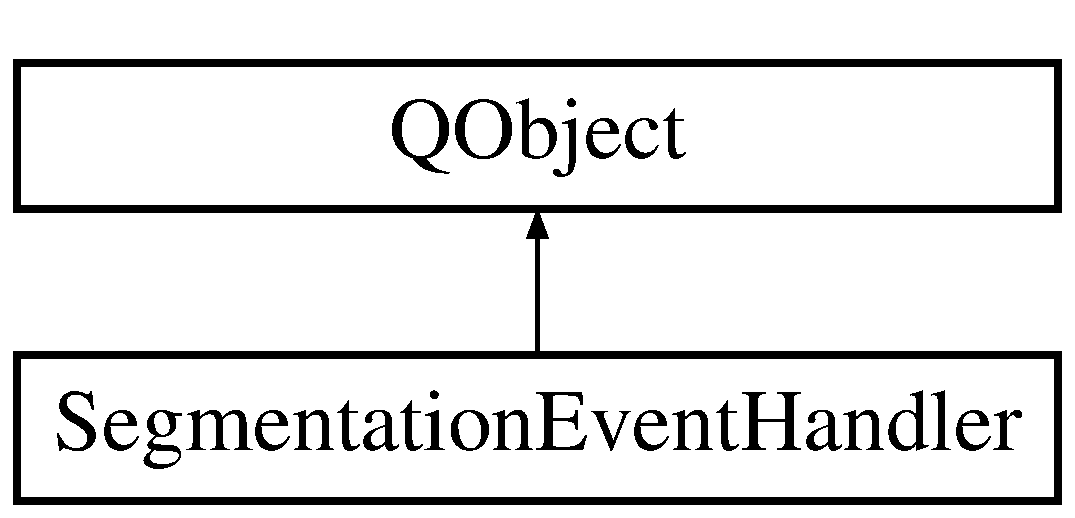
\includegraphics[height=2.000000cm]{classSegmentationEventHandler}
\end{center}
\end{figure}
\subsection*{Signals}
\begin{DoxyCompactItemize}
\item 
void \hyperlink{classSegmentationEventHandler_a7e0469cfa7b7de154a7f4ab89aa5d01c}{send\-Image} (const Q\-Image \&final\-Image)
\end{DoxyCompactItemize}
\subsection*{Public Member Functions}
\begin{DoxyCompactItemize}
\item 
\hyperlink{classSegmentationEventHandler_ae9ae201d2babf6d7a75039b1df9914ac}{Segmentation\-Event\-Handler} ()
\item 
\hyperlink{classSegmentationEventHandler_a0ed321c52deb44c8db76b0d100e8b614}{$\sim$\-Segmentation\-Event\-Handler} ()
\item 
Q\-Image \hyperlink{classSegmentationEventHandler_a40df09d50701ea6490b5ba6bb1841919}{load\-Image} (const string file\-Path)
\item 
void \hyperlink{classSegmentationEventHandler_a8111dd952df6dca9f13ac0aa6bf4105b}{segment} (const Q\-Image \&image, const Mat \&background\-Image, const Mat \&foreground\-Image, const double beta)
\item 
Q\-Image \hyperlink{classSegmentationEventHandler_adfa64d0cda9254629fea83982c0a22e2}{obtain\-Image\-With\-Boundary} (const Q\-Image \&input\-Image, const Q\-Image \&segmented\-Image)
\item 
bool \hyperlink{classSegmentationEventHandler_a2e82ef87339a521615c721e5706f69b9}{save\-Image} (const Q\-Image \&image, const Q\-String \&path)
\end{DoxyCompactItemize}


\subsection{Detailed Description}
This class handles the events of the U\-I classes.

\begin{DoxyAuthor}{Author}
Jose Bernal \& Rodrigo Daudt 
\end{DoxyAuthor}


\subsection{Constructor \& Destructor Documentation}
\hypertarget{classSegmentationEventHandler_ae9ae201d2babf6d7a75039b1df9914ac}{\index{Segmentation\-Event\-Handler@{Segmentation\-Event\-Handler}!Segmentation\-Event\-Handler@{Segmentation\-Event\-Handler}}
\index{Segmentation\-Event\-Handler@{Segmentation\-Event\-Handler}!SegmentationEventHandler@{Segmentation\-Event\-Handler}}
\subsubsection[{Segmentation\-Event\-Handler}]{\setlength{\rightskip}{0pt plus 5cm}Segmentation\-Event\-Handler\-::\-Segmentation\-Event\-Handler (
\begin{DoxyParamCaption}
{}
\end{DoxyParamCaption}
)}}\label{classSegmentationEventHandler_ae9ae201d2babf6d7a75039b1df9914ac}
Default constructor. \hypertarget{classSegmentationEventHandler_a0ed321c52deb44c8db76b0d100e8b614}{\index{Segmentation\-Event\-Handler@{Segmentation\-Event\-Handler}!$\sim$\-Segmentation\-Event\-Handler@{$\sim$\-Segmentation\-Event\-Handler}}
\index{$\sim$\-Segmentation\-Event\-Handler@{$\sim$\-Segmentation\-Event\-Handler}!SegmentationEventHandler@{Segmentation\-Event\-Handler}}
\subsubsection[{$\sim$\-Segmentation\-Event\-Handler}]{\setlength{\rightskip}{0pt plus 5cm}Segmentation\-Event\-Handler\-::$\sim$\-Segmentation\-Event\-Handler (
\begin{DoxyParamCaption}
{}
\end{DoxyParamCaption}
)}}\label{classSegmentationEventHandler_a0ed321c52deb44c8db76b0d100e8b614}
Class destructor. 

\subsection{Member Function Documentation}
\hypertarget{classSegmentationEventHandler_a40df09d50701ea6490b5ba6bb1841919}{\index{Segmentation\-Event\-Handler@{Segmentation\-Event\-Handler}!load\-Image@{load\-Image}}
\index{load\-Image@{load\-Image}!SegmentationEventHandler@{Segmentation\-Event\-Handler}}
\subsubsection[{load\-Image}]{\setlength{\rightskip}{0pt plus 5cm}Q\-Image Segmentation\-Event\-Handler\-::load\-Image (
\begin{DoxyParamCaption}
\item[{const string}]{file\-Path}
\end{DoxyParamCaption}
)}}\label{classSegmentationEventHandler_a40df09d50701ea6490b5ba6bb1841919}
Load image on file\-Path


\begin{DoxyParams}{Parameters}
{\em file\-Path} & path of the file to load\\
\hline
\end{DoxyParams}
\begin{DoxyReturn}{Returns}
Q\-Image loaded image 
\end{DoxyReturn}
\hypertarget{classSegmentationEventHandler_adfa64d0cda9254629fea83982c0a22e2}{\index{Segmentation\-Event\-Handler@{Segmentation\-Event\-Handler}!obtain\-Image\-With\-Boundary@{obtain\-Image\-With\-Boundary}}
\index{obtain\-Image\-With\-Boundary@{obtain\-Image\-With\-Boundary}!SegmentationEventHandler@{Segmentation\-Event\-Handler}}
\subsubsection[{obtain\-Image\-With\-Boundary}]{\setlength{\rightskip}{0pt plus 5cm}Q\-Image Segmentation\-Event\-Handler\-::obtain\-Image\-With\-Boundary (
\begin{DoxyParamCaption}
\item[{const Q\-Image \&}]{input\-Image, }
\item[{const Q\-Image \&}]{segmented\-Image}
\end{DoxyParamCaption}
)}}\label{classSegmentationEventHandler_adfa64d0cda9254629fea83982c0a22e2}
Returns the image with the boundary according to the segmentation image.


\begin{DoxyParams}{Parameters}
{\em input\-Image} & input image \\
\hline
{\em segmented\-Image} & binary image containing the segmentation of input image\\
\hline
\end{DoxyParams}
\begin{DoxyReturn}{Returns}
an image containing the respective boundaries. 
\end{DoxyReturn}
\hypertarget{classSegmentationEventHandler_a2e82ef87339a521615c721e5706f69b9}{\index{Segmentation\-Event\-Handler@{Segmentation\-Event\-Handler}!save\-Image@{save\-Image}}
\index{save\-Image@{save\-Image}!SegmentationEventHandler@{Segmentation\-Event\-Handler}}
\subsubsection[{save\-Image}]{\setlength{\rightskip}{0pt plus 5cm}bool Segmentation\-Event\-Handler\-::save\-Image (
\begin{DoxyParamCaption}
\item[{const Q\-Image \&}]{image, }
\item[{const Q\-String \&}]{path}
\end{DoxyParamCaption}
)}}\label{classSegmentationEventHandler_a2e82ef87339a521615c721e5706f69b9}
Load image on file\-Path


\begin{DoxyParams}{Parameters}
{\em image} & image to save \\
\hline
{\em file\-Path} & path to save the image\\
\hline
\end{DoxyParams}
\begin{DoxyReturn}{Returns}
true if the process was successful 
\end{DoxyReturn}
\hypertarget{classSegmentationEventHandler_a8111dd952df6dca9f13ac0aa6bf4105b}{\index{Segmentation\-Event\-Handler@{Segmentation\-Event\-Handler}!segment@{segment}}
\index{segment@{segment}!SegmentationEventHandler@{Segmentation\-Event\-Handler}}
\subsubsection[{segment}]{\setlength{\rightskip}{0pt plus 5cm}void Segmentation\-Event\-Handler\-::segment (
\begin{DoxyParamCaption}
\item[{const Q\-Image \&}]{image, }
\item[{const Mat \&}]{background\-Image, }
\item[{const Mat \&}]{foreground\-Image, }
\item[{const double}]{beta}
\end{DoxyParamCaption}
)}}\label{classSegmentationEventHandler_a8111dd952df6dca9f13ac0aa6bf4105b}
Calls the seededsegmentation class with the given inputs.


\begin{DoxyParams}{Parameters}
{\em image} & image to be segmented \\
\hline
{\em background\-Image} & background image to segment \\
\hline
{\em foreground\-Image} & foreground image to segment \\
\hline
{\em beta} & tuning variable \\
\hline
\end{DoxyParams}
\hypertarget{classSegmentationEventHandler_a7e0469cfa7b7de154a7f4ab89aa5d01c}{\index{Segmentation\-Event\-Handler@{Segmentation\-Event\-Handler}!send\-Image@{send\-Image}}
\index{send\-Image@{send\-Image}!SegmentationEventHandler@{Segmentation\-Event\-Handler}}
\subsubsection[{send\-Image}]{\setlength{\rightskip}{0pt plus 5cm}void Segmentation\-Event\-Handler\-::send\-Image (
\begin{DoxyParamCaption}
\item[{const Q\-Image \&}]{final\-Image}
\end{DoxyParamCaption}
)\hspace{0.3cm}{\ttfamily [signal]}}}\label{classSegmentationEventHandler_a7e0469cfa7b7de154a7f4ab89aa5d01c}
Signal emitted when the result after segmentation is obtained. 

The documentation for this class was generated from the following files\-:\begin{DoxyCompactItemize}
\item 
/home/jose/\-Documents/\-Seeded\-Image\-Segmentation\-Project/src/communication/segmentationeventhandler.\-h\item 
/home/jose/\-Documents/\-Seeded\-Image\-Segmentation\-Project/src/communication/moc\-\_\-segmentationeventhandler.\-cpp\item 
/home/jose/\-Documents/\-Seeded\-Image\-Segmentation\-Project/src/communication/segmentationeventhandler.\-cpp\end{DoxyCompactItemize}

\hypertarget{classSegmentationThread}{\section{Segmentation\-Thread Class Reference}
\label{classSegmentationThread}\index{Segmentation\-Thread@{Segmentation\-Thread}}
}


{\ttfamily \#include $<$segmentationthread.\-h$>$}

Inheritance diagram for Segmentation\-Thread\-:\begin{figure}[H]
\begin{center}
\leavevmode
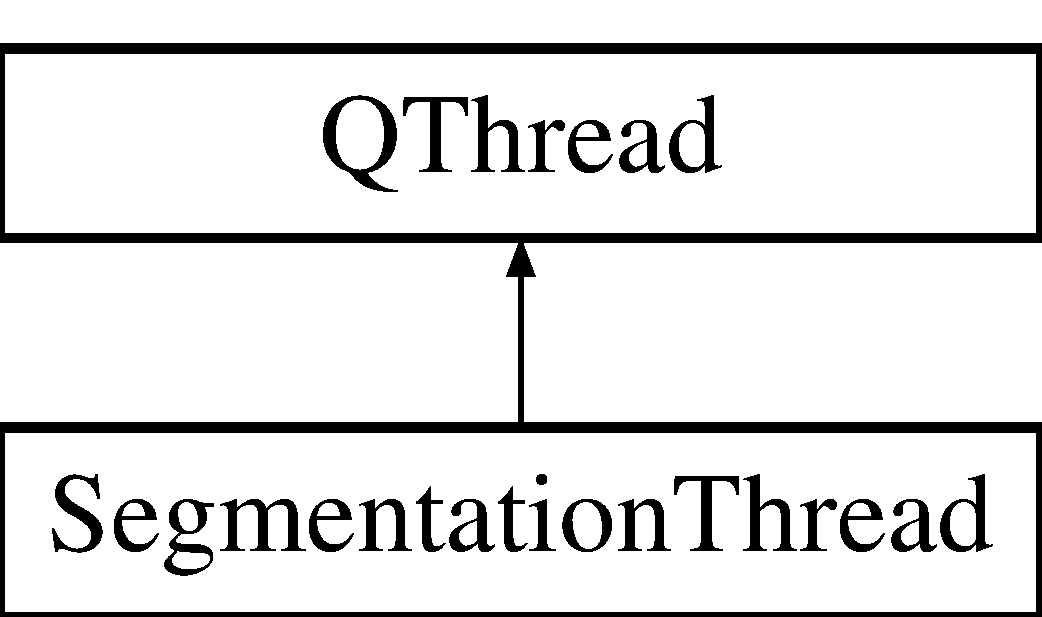
\includegraphics[height=2.000000cm]{classSegmentationThread}
\end{center}
\end{figure}
\subsection*{Signals}
\begin{DoxyCompactItemize}
\item 
void \hyperlink{classSegmentationThread_a2e74f10ff17d3f8d1c8d0767b6ff5e5e}{send\-Image} (const Mat \&image)
\end{DoxyCompactItemize}
\subsection*{Public Member Functions}
\begin{DoxyCompactItemize}
\item 
\hyperlink{classSegmentationThread_a5c5b9a1f21e114db574804220a7c2c21}{Segmentation\-Thread} ()
\item 
\hyperlink{classSegmentationThread_a3f8e826a615355c7ee2abb76601d2deb}{$\sim$\-Segmentation\-Thread} ()
\item 
void \hyperlink{classSegmentationThread_af901597e735165b6ef3b894826779eff}{process\-Image} (const Mat \&input\-Image, const Mat \&background\-Image, const Mat \&foreground\-Image, const \hyperlink{classNeighbourhood}{Neighbourhood} \&neighbourhood, const double beta)
\end{DoxyCompactItemize}
\subsection*{Protected Member Functions}
\begin{DoxyCompactItemize}
\item 
void \hyperlink{classSegmentationThread_ad98d9532eb60741d884849f26f62c38c}{run} ()
\end{DoxyCompactItemize}


\subsection{Detailed Description}
This class is in charge of the segmentation process.

\begin{DoxySeeAlso}{See Also}
\href{http://doc.qt.io/qt-5/qtcore-threads-queuedcustomtype-renderthread-h.html}{\tt http\-://doc.\-qt.\-io/qt-\/5/qtcore-\/threads-\/queuedcustomtype-\/renderthread-\/h.\-html}
\end{DoxySeeAlso}
\begin{DoxyAuthor}{Author}
Jose Bernal 
\end{DoxyAuthor}


\subsection{Constructor \& Destructor Documentation}
\hypertarget{classSegmentationThread_a5c5b9a1f21e114db574804220a7c2c21}{\index{Segmentation\-Thread@{Segmentation\-Thread}!Segmentation\-Thread@{Segmentation\-Thread}}
\index{Segmentation\-Thread@{Segmentation\-Thread}!SegmentationThread@{Segmentation\-Thread}}
\subsubsection[{Segmentation\-Thread}]{\setlength{\rightskip}{0pt plus 5cm}Segmentation\-Thread\-::\-Segmentation\-Thread (
\begin{DoxyParamCaption}
{}
\end{DoxyParamCaption}
)}}\label{classSegmentationThread_a5c5b9a1f21e114db574804220a7c2c21}
Default constructor. \hypertarget{classSegmentationThread_a3f8e826a615355c7ee2abb76601d2deb}{\index{Segmentation\-Thread@{Segmentation\-Thread}!$\sim$\-Segmentation\-Thread@{$\sim$\-Segmentation\-Thread}}
\index{$\sim$\-Segmentation\-Thread@{$\sim$\-Segmentation\-Thread}!SegmentationThread@{Segmentation\-Thread}}
\subsubsection[{$\sim$\-Segmentation\-Thread}]{\setlength{\rightskip}{0pt plus 5cm}Segmentation\-Thread\-::$\sim$\-Segmentation\-Thread (
\begin{DoxyParamCaption}
{}
\end{DoxyParamCaption}
)}}\label{classSegmentationThread_a3f8e826a615355c7ee2abb76601d2deb}
Class destructor. 

\subsection{Member Function Documentation}
\hypertarget{classSegmentationThread_af901597e735165b6ef3b894826779eff}{\index{Segmentation\-Thread@{Segmentation\-Thread}!process\-Image@{process\-Image}}
\index{process\-Image@{process\-Image}!SegmentationThread@{Segmentation\-Thread}}
\subsubsection[{process\-Image}]{\setlength{\rightskip}{0pt plus 5cm}void Segmentation\-Thread\-::process\-Image (
\begin{DoxyParamCaption}
\item[{const Mat \&}]{input\-Image, }
\item[{const Mat \&}]{background\-Image, }
\item[{const Mat \&}]{foreground\-Image, }
\item[{const {\bf Neighbourhood} \&}]{neighbourhood, }
\item[{const double}]{beta}
\end{DoxyParamCaption}
)}}\label{classSegmentationThread_af901597e735165b6ef3b894826779eff}
Calls the seededsegmentation class with the given inputs. This call is asynchronous. The result of this process is given by the slot


\begin{DoxyParams}{Parameters}
{\em image} & image to be segmented \\
\hline
{\em background\-Image} & background image to segment \\
\hline
{\em foreground\-Image} & foreground image to segment \\
\hline
{\em beta} & tuning variable \\
\hline
\end{DoxyParams}
\hypertarget{classSegmentationThread_ad98d9532eb60741d884849f26f62c38c}{\index{Segmentation\-Thread@{Segmentation\-Thread}!run@{run}}
\index{run@{run}!SegmentationThread@{Segmentation\-Thread}}
\subsubsection[{run}]{\setlength{\rightskip}{0pt plus 5cm}void Segmentation\-Thread\-::run (
\begin{DoxyParamCaption}
{}
\end{DoxyParamCaption}
)\hspace{0.3cm}{\ttfamily [protected]}}}\label{classSegmentationThread_ad98d9532eb60741d884849f26f62c38c}
Calls the segment method of \hyperlink{classSeededSegmentation}{Seeded\-Segmentation}. \hypertarget{classSegmentationThread_a2e74f10ff17d3f8d1c8d0767b6ff5e5e}{\index{Segmentation\-Thread@{Segmentation\-Thread}!send\-Image@{send\-Image}}
\index{send\-Image@{send\-Image}!SegmentationThread@{Segmentation\-Thread}}
\subsubsection[{send\-Image}]{\setlength{\rightskip}{0pt plus 5cm}void Segmentation\-Thread\-::send\-Image (
\begin{DoxyParamCaption}
\item[{const Mat \&}]{image}
\end{DoxyParamCaption}
)\hspace{0.3cm}{\ttfamily [signal]}}}\label{classSegmentationThread_a2e74f10ff17d3f8d1c8d0767b6ff5e5e}
Signal containing a the matrix with the segmentation 

The documentation for this class was generated from the following files\-:\begin{DoxyCompactItemize}
\item 
/home/jose/\-Documents/\-Seeded\-Image\-Segmentation\-Project/src/communication/segmentationthread.\-h\item 
/home/jose/\-Documents/\-Seeded\-Image\-Segmentation\-Project/src/communication/moc\-\_\-segmentationthread.\-cpp\item 
/home/jose/\-Documents/\-Seeded\-Image\-Segmentation\-Project/src/communication/segmentationthread.\-cpp\end{DoxyCompactItemize}

\hypertarget{classSegmentationUtility}{\section{Segmentation\-Utility Class Reference}
\label{classSegmentationUtility}\index{Segmentation\-Utility@{Segmentation\-Utility}}
}


{\ttfamily \#include $<$segmentationutility.\-h$>$}

\subsection*{Static Public Member Functions}
\begin{DoxyCompactItemize}
\item 
static Mat \hyperlink{classSegmentationUtility_a66410b9d63b6011d85a2d8bb0a79b614}{compute\-Boundary} (const Mat \&input\-Image)
\item 
static Mat \hyperlink{classSegmentationUtility_abeb1595a744a2083078895d49b7cafce}{multiply} (const Mat \&input\-Image, const cv\-::\-Scalar \&scalar)
\item 
static Mat \hyperlink{classSegmentationUtility_a6bb06eb4b8f16bb4ef2ce0c568324993}{normalized\-Image} (const Mat \&input\-Image)
\item 
static Mat \hyperlink{classSegmentationUtility_a199caf25d0ced552b4172d3b44123c48}{obtain\-Image\-With\-Boundary} (const Mat \&input\-Image, const Mat \&segmented\-Image)
\end{DoxyCompactItemize}


\subsection{Detailed Description}
This class present a set of utilities for polishing the segmentation result.

\begin{DoxyAuthor}{Author}
Rodrigo Daudt 
\end{DoxyAuthor}


\subsection{Member Function Documentation}
\hypertarget{classSegmentationUtility_a66410b9d63b6011d85a2d8bb0a79b614}{\index{Segmentation\-Utility@{Segmentation\-Utility}!compute\-Boundary@{compute\-Boundary}}
\index{compute\-Boundary@{compute\-Boundary}!SegmentationUtility@{Segmentation\-Utility}}
\subsubsection[{compute\-Boundary}]{\setlength{\rightskip}{0pt plus 5cm}Mat Segmentation\-Utility\-::compute\-Boundary (
\begin{DoxyParamCaption}
\item[{const Mat \&}]{input\-Image}
\end{DoxyParamCaption}
)\hspace{0.3cm}{\ttfamily [static]}}}\label{classSegmentationUtility_a66410b9d63b6011d85a2d8bb0a79b614}
Computes the boundary of the given binary image.


\begin{DoxyParams}{Parameters}
{\em input\-Image} & binary image to be processed.\\
\hline
\end{DoxyParams}
\begin{DoxyReturn}{Returns}
boundary obtained for the given image. 
\end{DoxyReturn}
\hypertarget{classSegmentationUtility_abeb1595a744a2083078895d49b7cafce}{\index{Segmentation\-Utility@{Segmentation\-Utility}!multiply@{multiply}}
\index{multiply@{multiply}!SegmentationUtility@{Segmentation\-Utility}}
\subsubsection[{multiply}]{\setlength{\rightskip}{0pt plus 5cm}Mat Segmentation\-Utility\-::multiply (
\begin{DoxyParamCaption}
\item[{const Mat \&}]{input\-Image, }
\item[{const cv\-::\-Scalar \&}]{scalar}
\end{DoxyParamCaption}
)\hspace{0.3cm}{\ttfamily [static]}}}\label{classSegmentationUtility_abeb1595a744a2083078895d49b7cafce}
Multiplies the given image by the given scalar.


\begin{DoxyParams}{Parameters}
{\em input\-Image} & image to be processed. \\
\hline
{\em scalar} & scalar to multiply\\
\hline
\end{DoxyParams}
\begin{DoxyReturn}{Returns}
the result of the multiplication 
\end{DoxyReturn}
\hypertarget{classSegmentationUtility_a6bb06eb4b8f16bb4ef2ce0c568324993}{\index{Segmentation\-Utility@{Segmentation\-Utility}!normalized\-Image@{normalized\-Image}}
\index{normalized\-Image@{normalized\-Image}!SegmentationUtility@{Segmentation\-Utility}}
\subsubsection[{normalized\-Image}]{\setlength{\rightskip}{0pt plus 5cm}Mat Segmentation\-Utility\-::normalized\-Image (
\begin{DoxyParamCaption}
\item[{const Mat \&}]{input\-Image}
\end{DoxyParamCaption}
)\hspace{0.3cm}{\ttfamily [static]}}}\label{classSegmentationUtility_a6bb06eb4b8f16bb4ef2ce0c568324993}
Obtain the normalized image from 0 to 1.


\begin{DoxyParams}{Parameters}
{\em input\-Image} & image to be processed.\\
\hline
\end{DoxyParams}
\begin{DoxyReturn}{Returns}
the normalized image 
\end{DoxyReturn}
\hypertarget{classSegmentationUtility_a199caf25d0ced552b4172d3b44123c48}{\index{Segmentation\-Utility@{Segmentation\-Utility}!obtain\-Image\-With\-Boundary@{obtain\-Image\-With\-Boundary}}
\index{obtain\-Image\-With\-Boundary@{obtain\-Image\-With\-Boundary}!SegmentationUtility@{Segmentation\-Utility}}
\subsubsection[{obtain\-Image\-With\-Boundary}]{\setlength{\rightskip}{0pt plus 5cm}Mat Segmentation\-Utility\-::obtain\-Image\-With\-Boundary (
\begin{DoxyParamCaption}
\item[{const Mat \&}]{input\-Image, }
\item[{const Mat \&}]{segmented\-Image}
\end{DoxyParamCaption}
)\hspace{0.3cm}{\ttfamily [static]}}}\label{classSegmentationUtility_a199caf25d0ced552b4172d3b44123c48}
Creates an image taking into account the input image and the segmented image. The result will show the input image and the boundary of the segmented regions.


\begin{DoxyParams}{Parameters}
{\em input\-Image} & image to be processed. \\
\hline
{\em segmented\-Image} & image resulting from the segmentation process.\\
\hline
\end{DoxyParams}
\begin{DoxyReturn}{Returns}
input image with boundary of the segmented regions. 
\end{DoxyReturn}


The documentation for this class was generated from the following files\-:\begin{DoxyCompactItemize}
\item 
/home/jose/\-Documents/\-Seeded\-Image\-Segmentation\-Project/src/common/segmentationutility.\-h\item 
/home/jose/\-Documents/\-Seeded\-Image\-Segmentation\-Project/src/common/segmentationutility.\-cpp\end{DoxyCompactItemize}

\hypertarget{classUi__MainWindow}{\section{Ui\-\_\-\-Main\-Window Class Reference}
\label{classUi__MainWindow}\index{Ui\-\_\-\-Main\-Window@{Ui\-\_\-\-Main\-Window}}
}
Inheritance diagram for Ui\-\_\-\-Main\-Window\-:\begin{figure}[H]
\begin{center}
\leavevmode
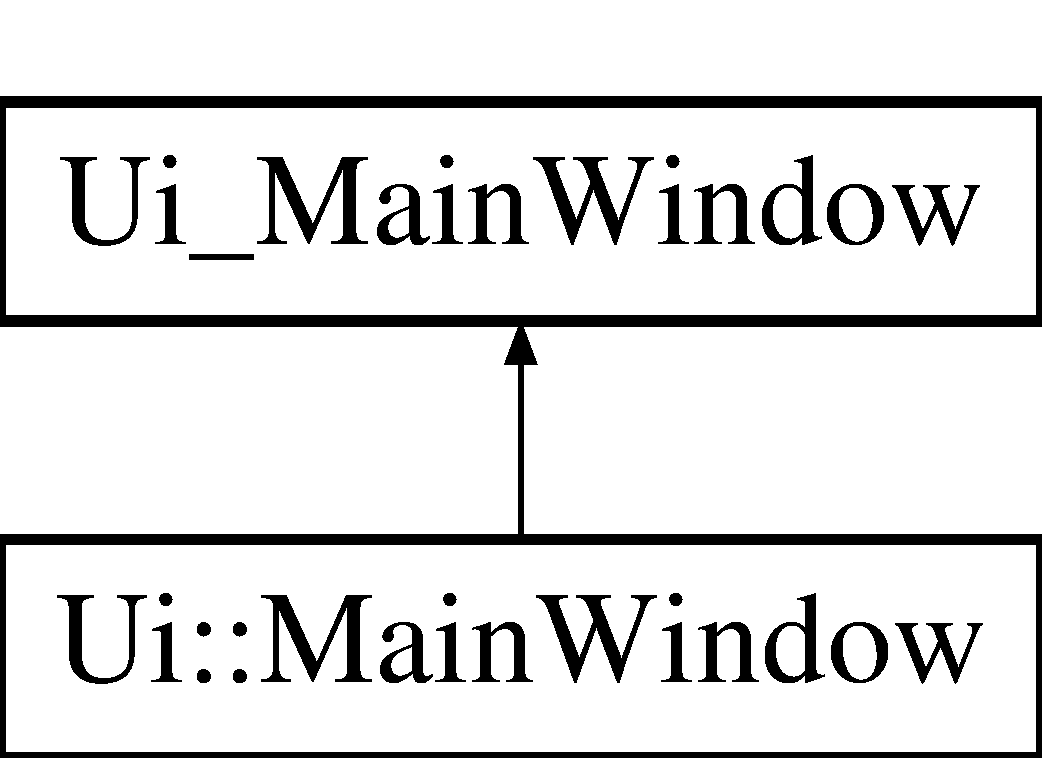
\includegraphics[height=2.000000cm]{classUi__MainWindow}
\end{center}
\end{figure}
\subsection*{Public Member Functions}
\begin{DoxyCompactItemize}
\item 
\hypertarget{classUi__MainWindow_acf4a0872c4c77d8f43a2ec66ed849b58}{void {\bfseries setup\-Ui} (Q\-Main\-Window $\ast$\hyperlink{classMainWindow}{Main\-Window})}\label{classUi__MainWindow_acf4a0872c4c77d8f43a2ec66ed849b58}

\item 
\hypertarget{classUi__MainWindow_a097dd160c3534a204904cb374412c618}{void {\bfseries retranslate\-Ui} (Q\-Main\-Window $\ast$\hyperlink{classMainWindow}{Main\-Window})}\label{classUi__MainWindow_a097dd160c3534a204904cb374412c618}

\end{DoxyCompactItemize}
\subsection*{Public Attributes}
\begin{DoxyCompactItemize}
\item 
\hypertarget{classUi__MainWindow_a30075506c2116c3ed4ff25e07ae75f81}{Q\-Widget $\ast$ {\bfseries central\-Widget}}\label{classUi__MainWindow_a30075506c2116c3ed4ff25e07ae75f81}

\item 
\hypertarget{classUi__MainWindow_a03ce63974cc69b067c91bbf285cceca8}{Q\-H\-Box\-Layout $\ast$ {\bfseries horizontal\-Layout\-\_\-3}}\label{classUi__MainWindow_a03ce63974cc69b067c91bbf285cceca8}

\item 
\hypertarget{classUi__MainWindow_a7871ea8c4b6c595d7ccd53960b344719}{Q\-Spacer\-Item $\ast$ {\bfseries horizontal\-Spacer}}\label{classUi__MainWindow_a7871ea8c4b6c595d7ccd53960b344719}

\item 
\hypertarget{classUi__MainWindow_aecd96a04789fcfec3f98d80390ad8184}{Q\-V\-Box\-Layout $\ast$ {\bfseries vertical\-Layout}}\label{classUi__MainWindow_aecd96a04789fcfec3f98d80390ad8184}

\item 
\hypertarget{classUi__MainWindow_a8384329c3663ff274e926a12024aab52}{Q\-Spacer\-Item $\ast$ {\bfseries vertical\-Spacer}}\label{classUi__MainWindow_a8384329c3663ff274e926a12024aab52}

\item 
\hypertarget{classUi__MainWindow_aff9ad585b5d6cd73c50b65a6a1104e77}{Q\-Push\-Button $\ast$ {\bfseries push\-Button\-Open\-Image}}\label{classUi__MainWindow_aff9ad585b5d6cd73c50b65a6a1104e77}

\item 
\hypertarget{classUi__MainWindow_adc1f5fdd97fb3729999c56902d0fa591}{Q\-Spacer\-Item $\ast$ {\bfseries vertical\-Spacer\-\_\-2}}\label{classUi__MainWindow_adc1f5fdd97fb3729999c56902d0fa591}

\item 
\hypertarget{classUi__MainWindow_acd6fdc9ebacc4b25b834162380d75ce8}{Q\-H\-Box\-Layout $\ast$ {\bfseries horizontal\-Layout}}\label{classUi__MainWindow_acd6fdc9ebacc4b25b834162380d75ce8}

\item 
\hypertarget{classUi__MainWindow_a71605bcf74c938f64207451850fc69b1}{Q\-Spacer\-Item $\ast$ {\bfseries horizontal\-Spacer\-\_\-5}}\label{classUi__MainWindow_a71605bcf74c938f64207451850fc69b1}

\item 
\hypertarget{classUi__MainWindow_a859ef6b7ed20c5dc3062f06678ef1e4c}{Q\-Push\-Button $\ast$ {\bfseries push\-Button\-Seed1}}\label{classUi__MainWindow_a859ef6b7ed20c5dc3062f06678ef1e4c}

\item 
\hypertarget{classUi__MainWindow_ae2007c6e48638f819d3ac57be8daa4ca}{Q\-Spacer\-Item $\ast$ {\bfseries horizontal\-Spacer\-\_\-3}}\label{classUi__MainWindow_ae2007c6e48638f819d3ac57be8daa4ca}

\item 
\hypertarget{classUi__MainWindow_a29ed28369fd46c711fea8c856f91577b}{Q\-Push\-Button $\ast$ {\bfseries push\-Button\-Seed2}}\label{classUi__MainWindow_a29ed28369fd46c711fea8c856f91577b}

\item 
\hypertarget{classUi__MainWindow_a3202b80ffde7629da626c1e0994f63f5}{Q\-Spacer\-Item $\ast$ {\bfseries horizontal\-Spacer\-\_\-6}}\label{classUi__MainWindow_a3202b80ffde7629da626c1e0994f63f5}

\item 
\hypertarget{classUi__MainWindow_a298e82ba0cc2500cd61f393f493e4529}{Q\-Spacer\-Item $\ast$ {\bfseries vertical\-Spacer\-\_\-4}}\label{classUi__MainWindow_a298e82ba0cc2500cd61f393f493e4529}

\item 
\hypertarget{classUi__MainWindow_abe535d626fd6aacbda232a4b72c8c8ae}{Q\-Push\-Button $\ast$ {\bfseries push\-Button\-Segment\-Image}}\label{classUi__MainWindow_abe535d626fd6aacbda232a4b72c8c8ae}

\item 
\hypertarget{classUi__MainWindow_a9d4bfb2fa0d87ccf9f7a311116676be6}{Q\-Spacer\-Item $\ast$ {\bfseries vertical\-Spacer\-\_\-5}}\label{classUi__MainWindow_a9d4bfb2fa0d87ccf9f7a311116676be6}

\item 
\hypertarget{classUi__MainWindow_a80867018070156432923d0266cc9fe25}{Q\-H\-Box\-Layout $\ast$ {\bfseries horizontal\-Layout\-\_\-2}}\label{classUi__MainWindow_a80867018070156432923d0266cc9fe25}

\item 
\hypertarget{classUi__MainWindow_acdff0826006698f82a7ef284f2950409}{Q\-Spacer\-Item $\ast$ {\bfseries horizontal\-Spacer\-\_\-7}}\label{classUi__MainWindow_acdff0826006698f82a7ef284f2950409}

\item 
\hypertarget{classUi__MainWindow_afca82fb141fba22818217db0e6bdd1df}{Q\-Push\-Button $\ast$ {\bfseries push\-Button\-\_\-save\-Binary}}\label{classUi__MainWindow_afca82fb141fba22818217db0e6bdd1df}

\item 
\hypertarget{classUi__MainWindow_a4fc05b11984637298795a354792c4023}{Q\-Spacer\-Item $\ast$ {\bfseries horizontal\-Spacer\-\_\-4}}\label{classUi__MainWindow_a4fc05b11984637298795a354792c4023}

\item 
\hypertarget{classUi__MainWindow_a6c72954e07c555c318c31c88c9a701bb}{Q\-Push\-Button $\ast$ {\bfseries push\-Button\-\_\-save\-Contour}}\label{classUi__MainWindow_a6c72954e07c555c318c31c88c9a701bb}

\item 
\hypertarget{classUi__MainWindow_a100e0ffd031f76754eba5078288deabf}{Q\-Spacer\-Item $\ast$ {\bfseries horizontal\-Spacer\-\_\-8}}\label{classUi__MainWindow_a100e0ffd031f76754eba5078288deabf}

\item 
\hypertarget{classUi__MainWindow_ac845bdf6b5b5237378a7b067808b7a31}{Q\-Spacer\-Item $\ast$ {\bfseries vertical\-Spacer\-\_\-3}}\label{classUi__MainWindow_ac845bdf6b5b5237378a7b067808b7a31}

\item 
\hypertarget{classUi__MainWindow_a9a022556cf8ce3fa47e51d79cb222ab0}{Q\-Spacer\-Item $\ast$ {\bfseries horizontal\-Spacer\-\_\-2}}\label{classUi__MainWindow_a9a022556cf8ce3fa47e51d79cb222ab0}

\item 
\hypertarget{classUi__MainWindow_a5172877001c8c7b4e0f6de50421867d1}{Q\-Tool\-Bar $\ast$ {\bfseries main\-Tool\-Bar}}\label{classUi__MainWindow_a5172877001c8c7b4e0f6de50421867d1}

\item 
\hypertarget{classUi__MainWindow_a50fa481337604bcc8bf68de18ab16ecd}{Q\-Status\-Bar $\ast$ {\bfseries status\-Bar}}\label{classUi__MainWindow_a50fa481337604bcc8bf68de18ab16ecd}

\end{DoxyCompactItemize}


The documentation for this class was generated from the following file\-:\begin{DoxyCompactItemize}
\item 
/home/jose/\-Documents/\-Seeded\-Image\-Segmentation\-Project/src/gui/ui\-\_\-mainwindow.\-h\end{DoxyCompactItemize}

\hypertarget{classUserInputException}{\section{User\-Input\-Exception Class Reference}
\label{classUserInputException}\index{User\-Input\-Exception@{User\-Input\-Exception}}
}


{\ttfamily \#include $<$userinputexception.\-h$>$}

Inheritance diagram for User\-Input\-Exception\-:\begin{figure}[H]
\begin{center}
\leavevmode
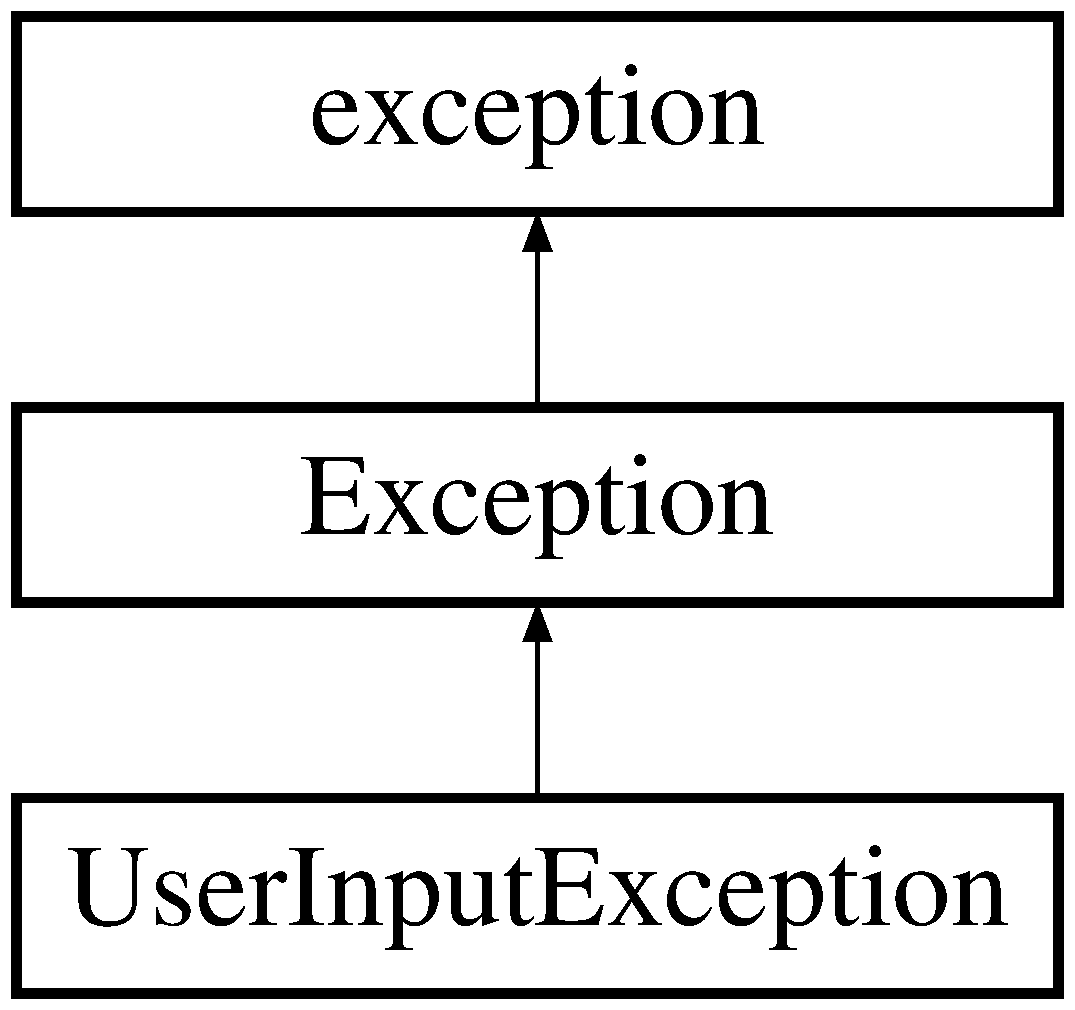
\includegraphics[height=3.000000cm]{classUserInputException}
\end{center}
\end{figure}
\subsection*{Public Member Functions}
\begin{DoxyCompactItemize}
\item 
\hyperlink{classUserInputException_a7b49a44bbab637d36a97bbf916e7ce85}{User\-Input\-Exception} (const string \hyperlink{classException_a3d5051a55e7133196d3097a5cd2d58a7}{message})
\end{DoxyCompactItemize}
\subsection*{Additional Inherited Members}


\subsection{Detailed Description}
This class represents the exceptions that have place when the inputs are not the expected.

\begin{DoxyAuthor}{Author}
Jose Bernal 
\end{DoxyAuthor}


\subsection{Constructor \& Destructor Documentation}
\hypertarget{classUserInputException_a7b49a44bbab637d36a97bbf916e7ce85}{\index{User\-Input\-Exception@{User\-Input\-Exception}!User\-Input\-Exception@{User\-Input\-Exception}}
\index{User\-Input\-Exception@{User\-Input\-Exception}!UserInputException@{User\-Input\-Exception}}
\subsubsection[{User\-Input\-Exception}]{\setlength{\rightskip}{0pt plus 5cm}User\-Input\-Exception\-::\-User\-Input\-Exception (
\begin{DoxyParamCaption}
\item[{const string}]{message}
\end{DoxyParamCaption}
)}}\label{classUserInputException_a7b49a44bbab637d36a97bbf916e7ce85}
Default constructor of the class


\begin{DoxyParams}{Parameters}
{\em message} & Message to display \\
\hline
\end{DoxyParams}


The documentation for this class was generated from the following files\-:\begin{DoxyCompactItemize}
\item 
/home/jose/\-Documents/\-Seeded\-Image\-Segmentation\-Project/src/exceptions/userinputexception.\-h\item 
/home/jose/\-Documents/\-Seeded\-Image\-Segmentation\-Project/src/exceptions/userinputexception.\-cpp\end{DoxyCompactItemize}

%--- End generated contents ---

% Index
\newpage
\phantomsection
\addcontentsline{toc}{chapter}{Index}
\printindex

\end{document}
